\documentclass[
11pt, % The default document font size, options: 10pt, 11pt, 12pt
%codirector, % Uncomment to add a codirector to the title page
]{charter} 

% El títulos de la memoria, se usa en la carátula y se puede usar el cualquier lugar del documento con el comando \ttitle
\titulo{Predicción de quiebra de empresas mediante técnicas de Machine Learning} 

% Nombre del posgrado, se usa en la carátula y se puede usar el cualquier lugar del documento con el comando \degreename
%\posgrado{Carrera de Especialización en Sistemas Embebidos} 
%\posgrado{Carrera de Especialización en Internet de las Cosas} 
\posgrado{Carrera de Especialización en Inteligencia Artificial}
%\posgrado{Maestría en Sistemas Embebidos} 
%\posgrado{Maestría en Internet de las cosas}

% Tu nombre, se puede usar el cualquier lugar del documento con el comando \authorname
% IMPORTANTE: no omitir titulaciones ni tildación en los nombres, también se recomienda escribir los nombres completos (tal cual los tienen en su documento)
\autor{Ing. Gaspar Acevedo Zain}

% El nombre del director y co-director, se puede usar el cualquier lugar del documento con el comando \supname y \cosupname y \pertesupname y \pertecosupname
\director{Título y Nombre del director}
\pertenenciaDirector{pertenencia} 
\codirector{} % para que aparezca en la portada se debe descomentar la opción codirector en los parámetros de documentclass
\pertenenciaCoDirector{FIUBA}

% Nombre del cliente, quien va a aprobar los resultados del proyecto, se puede usar con el comando \clientename y \empclientename
\cliente{Nombre del cliente}
\empresaCliente{Empresa del cliente}
 
\fechaINICIO{24 de junio de 2025}		%Fecha de inicio de la cursada de GdP \fechaInicioName
\fechaFINALPlan{19 de agosto de 2025} 	%Fecha de final de cursada de GdP
\fechaFINALTrabajo{a definir}	%Fecha de defensa pública del trabajo final

\usepackage{hyperref}
\usepackage{xltabular}
\usepackage{pdflscape}

\begin{document}

\maketitle
\thispagestyle{empty}
\pagebreak


\thispagestyle{empty}
{\setlength{\parskip}{0pt}
\tableofcontents{}
}
\pagebreak


\section*{Registros de cambios}
\label{sec:registro}


\begin{table}[ht]
\label{tab:registro}
\centering
\begin{tabularx}{\linewidth}{@{}|c|X|c|@{}}
\hline
\rowcolor[HTML]{C0C0C0} 
Revisión & \multicolumn{1}{c|}{\cellcolor[HTML]{C0C0C0}Detalles de los cambios realizados} & Fecha      \\ \hline
0      & Creación del documento                                 &\fechaInicioName \\ \hline
1      & Se completa hasta el punto 5 inclusive                & {6} de {Julio} de 2025 \\ \hline
2      & Se completa hasta el punto 9 inclusive                & {15} de {Julio} de 2025 \\ \hline
3      & Se completa hasta el punto 12 inclusive                & {29} de {Julio} de 2025 \\ \hline
%		  Se puede agregar algo más \newline
%		  En distintas líneas \newline
%		  Así                                                    & {día} de {mes} de 202X \\ \hline
%3      & Se completa hasta el punto 12 inclusive                & {día} de {mes} de 202X \\ \hline
%4      & Se completa el plan	                                 & {día} de {mes} de 202X \\ \hline

% Si hay más correcciones pasada la versión 4 también se deben especificar acá

\end{tabularx}
\end{table}

\pagebreak



\section*{Acta de constitución del proyecto}
\label{sec:acta}

\begin{flushright}
Buenos Aires, \fechaInicioName
\end{flushright}

\vspace{2cm}

Por medio de la presente se acuerda con el \authorname\hspace{1px} que su Trabajo Final de la \degreename\hspace{1px} se titulará ``\ttitle'' y consistirá en {el desarrollo de una herramienta basada en Machine Learning que permitirá predecir si una empresa puede entrar en quiebra o no}. El trabajo tendrá un presupuesto preliminar estimado de {604} horas y un costo estimado de \textcolor{red}{\$ XXX}, con fecha de inicio el \fechaInicioName\hspace{1px} y fecha de presentación pública el \fechaFinalName.

Se adjunta a esta acta la planificación inicial.

\vfill

% Esta parte se construye sola con la información que hayan cargado en el preámbulo del documento y no debe modificarla
\begin{table}[ht]
\centering
\begin{tabular}{ccc}
\begin{tabular}[c]{@{}c@{}}Dr. Ing. Ariel Lutenberg \\ Director posgrado FIUBA\end{tabular} & \hspace{2cm} & \begin{tabular}[c]{@{}c@{}}\clientename \\ \empclientename \end{tabular} \vspace{2.5cm} \\ 
\multicolumn{3}{c}{\begin{tabular}[c]{@{}c@{}} \supname \\ Director del Trabajo Final\end{tabular}} \vspace{2.5cm} \\
\end{tabular}
\end{table}


\section{1. Descripción técnica-conceptual del proyecto a realizar}
\label{sec:descripcion}

%\begin{consigna}{red} % ELIMINAR \begin{consigna}{red} y \end{consigna}{red} en las secciones que vayan completando para cada entrega parcial.
Este proyecto consiste en un emprendimiento personal cuyo objetivo es utilizar técnicas de aprendizaje de máquina para detectar si una empresa puede entrar en quiebra o no. Este tipo de análisis puede resultar de gran interés y utilidad para distintos actores del mercado financiero, tales como bancos, compañías aseguradoras, fondos de inversión o consultoras especializadas en riesgo crediticio. Por ello, estos se considerarán como potenciales clientes.

Para llevarlo a cabo, se utilizará un \textit{dataset} publicado por el \href{https://www.tejwin.com/en/}{Taiwan Economic Journal}, que contiene información financiera de empresas del mercado de Taiwán entre los años 1999 y 2009. Al ser estos datos públicos, hoy en día existen soluciones que exploran esta temática. Algunas de ellas hacen uso de modelos de \textit{machine learning} tales como \textit{SVM} y \textit{XGBoost}, junto con algunas técnicas de preprocesamiento de datos como \textit{Smote} y de búsqueda de hiperparámetros como \textit{Random Search}.

Con el fin de diferenciarse de estas soluciones, se propone implementar el marco de trabajo basado en \textit{MLFlow} definido en la figura \ref{fig:diagBloques}. Se detalla una serie de etapas cuyas salidas se refinarán durante distintas iteraciones. Esto permitirá a los usuarios finales trabajar en un entorno seguro, robusto, y reproducible.

El proyecto se encuentra en la etapa de planificación. El desarrollo e implementación se realizará en distintas etapas. Se comenzará con un análisis exploratorio de datos, que nos permitirá conocer mejor al dataset en cuestión. Luego, se realizarán iteraciones sobre las siguientes etapas:

\begin{itemize}
	\item Preprocesamiento de datos: en la primer iteración se implementarán técnicas de tratamiento de nulos y desbalance de clases. En las siguientes iteraciones, se estudiarán técnicas de extracción e ingeniería de features.
	\item Entrenamiento de modelos: se implementará un modelo distinto en cada iteración. Los modelos a explorar son regresión logística, \textit{SVM} y \textit{XGBoost}. También, se explorará la optimización de hiperparámetros mediante búsqueda bayesiana.
	\item Evaluación y refinamiento: en esta etapa se evaluará al modelo entrenado en la etapa anterior. Se generarán métricas que permitirán compararlo con resultados obtenidos en otras iteraciones.
\end{itemize}

La innovación de este proyecto radica en el uso del marco de trabajo definido en la figura \ref{fig:diagBloques}. Éste proporciona un ambiente productivo, reproducible y escalable, en donde se podrán analizar diversas técnicas de aprendizaje de máquina para detectar si una empresa puede entrar en quiebra o no.

\begin{figure}[htpb]
\centering 
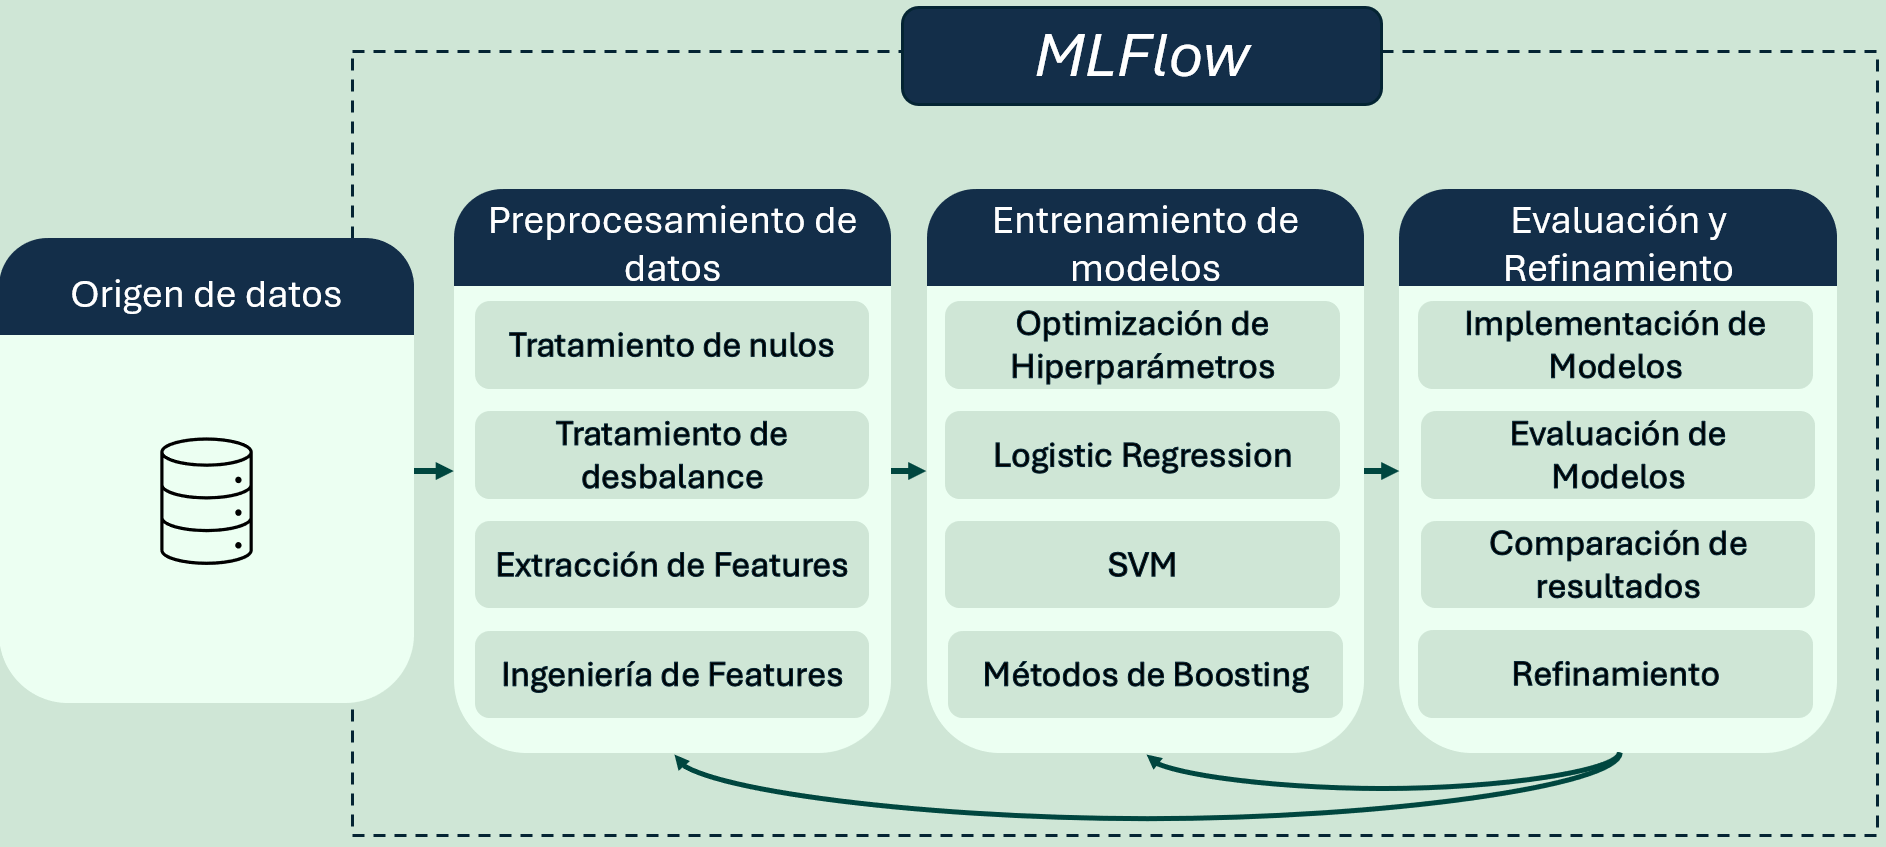
\includegraphics[width=.65\textwidth]{./Figuras/diagrama_bloques.png}
\caption{Diagrama en bloques del sistema.}
\label{fig:diagBloques}
\end{figure}

\vspace{25px}
%\end{consigna} % ELIMINAR \begin{consigna}{red} y \end{consigna}{red} en las secciones que vayan completando para cada entrega parcial.

\section{2. Identificación y análisis de los interesados}
\label{sec:interesados}

\begin{table}[ht]
%\caption{Identificación de los interesados}
%\label{tab:interesados}
\begin{tabularx}{\linewidth}{@{}|l|X|X|l|@{}}
\hline
\rowcolor[HTML]{C0C0C0} 
Rol           & Nombre y Apellido & Organización 	& Puesto 	\\ \hline
Responsable   & \authorname       & FIUBA        	& Alumno 	\\ \hline
Orientador    & \supname	      & \pertesupname 	& Director del Trabajo Final \\ \hline
Cliente & Actores del mercado financiero                   & -             	& -       	\\ \hline
Usuario final & Trabajadores de clientes                   & -             	& -       	\\ \hline
\end{tabularx}
\end{table}

\begin{itemize}
	\item Orientador: podrán ayudar en la recomendación y evaluación de técnicas a explorar en las diferentes etapas del proyecto.
	\item Cliente: si bien es un proyecto personal, se considerarán como potenciales clientes a distintos actores del mercado financiero, tales como bancos, compañías aseguradoras, fondos de inversión o consultoras especializadas en riesgo crediticio.
    \item Usuario final: analistas de riesgos, ejecutivo de créditos, entre otros integrantes que trabajan para los potenciales clientes.
\end{itemize}

\section{3. Propósito del proyecto}
\label{sec:proposito}

Predecir si una empresa puede entrar en quiebra o no, al explorar técnicas de \textit{machine learning} en un marco de trabajo productivo, reproducible y escalable.

\section{4. Alcance del proyecto}
\label{sec:alcance}

El alcance del proyecto incluye:
\begin{itemize}
	\item Análisis exploratorio de datos: se analizarán las distintas variables presentes en el \textit{dataset} de estudio, con el fin de conocer sus características y poder tomar decisiones con base en ellas.
    \item Preprocesamiento de datos: se realizarán técnicas de tratamiento de datos faltantes, selección y/o extracción de variables, como así también de ingeniería de features.
    \item Implementación de modelos de \textit{machine learning}: se estudiarán diversos modelos de aprendizaje de máquina sobre los datos procesados, tales como \textit{logistic regression}, \textit{SVM} y \textit{XGBoost}. Además, se optimizarán los hiperparámetros de estos modelos mediante búsqueda bayesiana.
    \item Evaluación y comparación de modelos: se obtendrán métricas relacionadas a los modelos explorados, con el fin de poder determinar cuál de ellos realiza una mejor predicción.
    \item Implementación de un entorno basado en \textit{MLFlow}: este entornó facilitará la realización, la reproducibilidad y la escalabilidad de las distintas etapas de trabajo que se realizarán en este proyecto. Este será de caracter local, es decir, no se implementará en una plataforma de \textit{cloud computing}.
\end{itemize}

No se incluye:
\begin{itemize}
    \item El despliegue del entorno de trabajo en una plataforma de \textit{cloud computing}, tales como \textit{Azure}, \textit{AWS}, entre otros.
    \item El análisis de otros \textit{datasets} distintos al propuesto.
\end{itemize}

\section{5. Supuestos del proyecto}
\label{sec:supuestos}

Para el desarrollo del presente proyecto se supone que:
\begin{itemize}
	\item Supuesto 1: el \textit{dataset} de estudio presenta datos fiables, y no tiene restricciones en cuanto a licencias de uso.
	\item Supuesto 2: una \textit{laptop} como equipo de trabajo es más que suficiente para realizar el preprocesamiento y entrenamiento de los modelos de aprendizaje automático.
	\item Supuesto 3: el entorno de \textit{MLFlow} podrá desarrollarse en etapas futuras del proyecto, posteriores a la exploración de los modelos de aprendizaje automático.
    \item Supuesto 4: el entorno de \textit{MLFlow} podrá desplegarse de manera local, sin necesidad de recurrir a plataforma de \textit{cloud computing}, tales como \textit{Azure}, \textit{AWS}, entre otros.
    \item Supuesto 5: se disponen de al menos 15 horas semanales para realizar el proyecto.
\end{itemize}

\section{6. Product Backlog}
\label{sec:backlog}
\textbf{Roles}
\begin{itemize}
    \item \textit{Ingeniero del proyecto}: es quien se encarga del análisis, diseño, desarrollo y despliegue del proyecto.
    \item \textit{Usuario final}: es quien consulta y analiza las predicciones de los modelos explorados en el proyecto.
\end{itemize}

\textbf{Criterios de ponderación de historias de usuario}

Esto son los criterios que se utilizan para ponderar a las historias de usuario mediante \textit{Story Points}:
\begin{itemize}
    \item Dificultad: representa la cantidad de trabajo estimado que requiere la historia de usuario para realizarse.
    \item Complejidad: representa la dificultad de realizar la historia de usuario a nivel técnico.
    \item Incertidumbre: representa el riesgo asociado a la historia de usuario.
\end{itemize}

Cada criterio tiene asociado las ponderaciones \textit{baja}, \textit{media} y \textit{alta}, que se detallan en el cuadro \ref{table:ponderaciones}. Los \textit{Story Points} de una historia de usuario quedan definidos por la suma de los valores de estas ponderaciones redondeada hacia el número superior más próximo en la serie de \textit{Fibonacci}.

\begin{table}[htpb]
\centering
\begin{tabular}{|c|c|c|c|}
\hline
\rowcolor[HTML]{C0C0C0}
Criterio\textbackslash Ponderación & Baja & Media & Alta \\ \hline
Dificultad & 1 & 3 & 5 \\ \hline
Complejidad & 1 & 3 & 5 \\ \hline
Incertidumbre & 1 & 5 & 8 \\ \hline
\end{tabular}
\caption{Tabla de ponderaciones de historia de usuario.}
\label{table:ponderaciones}
\end{table}

\textbf{\'{E}picas}
\begin{itemize}
  \item \textbf{\'{E}pica 1 - Análisis y procesamiento de datos}
    \begin{itemize}
      \item HU1 - Análisis exploratorio
        \begin{itemize}
            \item Como ingeniero del proyecto, quiero realizar un análisis exploratorio de datos para conocer las distribuciones, formas y otras particularidades de las variables del dataset con el que se trabajará.
            \item Ponderación
            \begin{itemize}
                \item Dificultad: media - 3 \textit{Story Points}
                \item Complejidad: baja - 1 \textit{Story Points}
                \item Incertidumbre: baja - 1 \textit{Story Points}
                \item Suma: 5
                \item Total: 5 \textit{Story Points}
            \end{itemize}            
        \end{itemize}
      \item HU2 - Procesamiento de datos faltantes y datos atípicos
        \begin{itemize}
            \item Como ingeniero del proyecto, quiero realizar un procesamiento de datos faltantes y de datos atípicos con el fin de asegurar la calidad del dataset.
            \item Ponderación
            \begin{itemize}
                \item Dificultad: media - 3 \textit{Story Points}
                \item Complejidad: media - 3 \textit{Story Points}
                \item Incertidumbre: baja - 1 \textit{Story Points}
                \item Suma: 7
                \item Total: 8 \textit{Story Points}
            \end{itemize}
        \end{itemize}
\newpage
      \item HU3 - \textit{Feature Engineering}
        \begin{itemize}
            \item Como ingeniero del proyecto, quiero implementar \textit{Feature Engineering} con el fin de crear nuevos atributos en el dataset.
            \item Ponderación
            \begin{itemize}
                \item Dificultad: media - 3 \textit{Story Points}
                \item Complejidad: media - 3 \textit{Story Points}
                \item Incertidumbre: baja - 1 \textit{Story Points}
                \item Suma: 7 
                \item Total: 8 \textit{Story Points}
            \end{itemize}
        \end{itemize}
    \end{itemize}
  \item \textbf{\'{E}pica 2 - Implementación y comparación de modelos}
    \begin{itemize}
      \item HU4 - Implementación de modelos de \textit{Machine Learning}
        \begin{itemize}
            \item Como ingeniero del proyecto, quiero implementar los modelos de \textit{Machine Learning} de \textit{Logistic Regression}, \textit{SVM} y \textit{XGBoost} que permitan predecir si una empresa entra en quiebra o no.
            \item Ponderación
            \begin{itemize}
                \item Dificultad: media - 3 \textit{Story Points}
                \item Complejidad: media - 3 \textit{Story Points}
                \item Incertidumbre: media - 5 \textit{Story Points}
                \item Suma: 11
                \item Total: 13 \textit{Story Points}
            \end{itemize}
        \end{itemize}
      \item HU5 - Optimización de hiperparámetros
        \begin{itemize}
            \item Como ingeniero del proyecto, quiero implementar técnicas de optimización de hiperparámetros y aplicarlas a los modelos de \textit{Machine Learning} implementados.
            \item Ponderación
            \begin{itemize}
                \item Dificultad: media - 3 \textit{Story Points}
                \item Complejidad: media - 3 \textit{Story Points}
                \item Incertidumbre: media - 5 \textit{Story Points}
                \item Suma: 11
                \item Total: 13 \textit{Story Points}
            \end{itemize}
        \end{itemize}
      \item HU6 - Métricas de modelos
        \begin{itemize}
            \item Como ingeniero del proyecto, quiero calcular las métricas de \textit{AUC-ROC} y \textit{F1-score} en cada modelo de \textit{Machine Learning} implementado y comparar sus resultados.
            \item Ponderación
            \begin{itemize}
                \item Dificultad: media - 3 \textit{Story Points}
                \item Complejidad: media - 3 \textit{Story Points}
                \item Incertidumbre: baja - 1 \textit{Story Points}
                \item Suma: 7
                \item Total: 8 \textit{Story Points}
            \end{itemize}
        \end{itemize}
    \end{itemize}
\newpage    
  \item \textbf{\'{E}pica 3 - Despliegue en entorno \textit{MLFlow}}
    \begin{itemize}
      \item HU7 - Despliegue en \textit{MLFlow}
        \begin{itemize}
            \item Como ingeniero del proyecto, quiero desplegar un entorno local de \textit{MLFLow} en donde se repliquen los pasos de procesamiento de datos e implementación y comparación de modelos.
            \item Ponderación
            \begin{itemize}
                \item Dificultad: alta - 5 \textit{Story Points}
                \item Complejidad: media - 3 \textit{Story Points}
                \item Incertidumbre: media - 5 \textit{Story Points}
                \item Suma: 13
                \item Total: 13 \textit{Story Points}
            \end{itemize}
        \end{itemize}
      \item HU8 - \textit{API} para entorno \textit{MLFlow}
        \begin{itemize}
            \item Como ingeniero del proyecto, quiero exponer el entorno de \textit{MLFlow} mediante una \textit{API} para facilitar el acceso y su utilización.
            \item Ponderación
            \begin{itemize}
                \item Dificultad: baja - 1 \textit{Story Points}
                \item Complejidad: media - 3 \textit{Story Points}
                \item Incertidumbre: baja - 1 \textit{Story Points}
                \item Suma: 5
                \item Total: 5 \textit{Story Points}
            \end{itemize}
        \end{itemize}
    \end{itemize}
  \item \textbf{\'{E}pica 4 - Gestión de calidad del código fuente}
    \begin{itemize}
      \item HU9 - Implementación de buenas prácticas
        \begin{itemize}
            \item Como ingeniero del proyecto, quiero asegurar que el código siga las buenas prácticas y estándares de la industria.
            \item Ponderación
            \begin{itemize}
                \item Dificultad: media - 3 \textit{Story Points}
                \item Complejidad: baja - 1 \textit{Story Points}
                \item Incertidumbre: baja - 1 \textit{Story Points}
                \item Suma: 5
                \item Total: 5 \textit{Story Points}
            \end{itemize}
        \end{itemize}
      \item HU10 - Documentación
        \begin{itemize}
            \item Como ingeniero del proyecto, quiero documentar todos los pasos realizados durante el proyecto.
            \item Ponderación
            \begin{itemize}
                \item Dificultad: baja - 1 \textit{Story Points}
                \item Complejidad: baja - 1 \textit{Story Points}
                \item Incertidumbre: baja - 1 \textit{Story Points}
                \item Suma: 3
                \item Total: 3 \textit{Story Points}
            \end{itemize}
        \end{itemize}
\newpage        
      \item HU11 - Validación de \textit{API} de \textit{MLFlow}
        \begin{itemize}
            \item Como usuario final, quiero consultar los resultados y comparaciones de los modelos mediante la \textit{API} del entorno de \textbf{MLFlow}, para poder analizarlos.
            \item Ponderación
            \begin{itemize}
                \item Dificultad: media - 3 \textit{Story Points}
                \item Complejidad: baja - 1 \textit{Story Points}
                \item Incertidumbre: baja - 1 \textit{Story Points}
                \item Suma: 5
                \item Total: 5 \textit{Story Points}
            \end{itemize}
        \end{itemize}        
    \end{itemize}
\end{itemize}

\section{7. Criterios de aceptación de historias de usuario}
\label{sec:criteriosAceptacion}

\begin{itemize}
  \item \textbf{\'{E}pica 1 - Análisis y procesamiento de datos}
    \begin{itemize}
      \item Criterios de aceptación HU1 - Análisis exploratorio
        \begin{itemize}
            \item Se estudia la presencia de datos atípicos y de datos faltantes para cada variable.
            \item Se grafican las distribuciones de las variables del dataset.
            \item Se realiza un estudio de correlaciones entre variables numéricas.
            \item Se documentan los hallazgos del análisis de cada variable.
        \end{itemize}
      \item Criterios de aceptación HU2 - Procesamiento de datos faltantes y datos atípicos
        \begin{itemize}
            \item Se realiza una imputación de datos faltantes a las variables del dataset.
            \item Se justifican los métodos de imputación utilizados.
            \item Se ajustan los datos atípicos de las variables del dataset.
            \item Se justifican los métodos de ajuste utilizados.
            \item Se justifican los casos en donde se decide no imputar ni ajustar.
        \end{itemize}
      \item Criterios de aceptación HU3 - \textit{Feature Engineering}
        \begin{itemize}
            \item Se crean nuevas variables en el dataset a partir de las existentes.
            \item Se estudia el impacto por separado de estas variables en los modelos generados, a partir de sus métricas.
            \item Se justifica la inclusión o no en el modelo de cada variable generada.
        \end{itemize}
    \end{itemize}
  \item \textbf{\'{E}pica 2 - Implementación y comparación de modelos}
    \begin{itemize}
      \item Criterios de aceptación HU4 - Implementación de modelos de \textit{Machine Learning}
        \begin{itemize}
            \item Se implementan distintos modelos de \textit{Machine Learning}.
            \item Se justifica el uso de cada uno de los modelos implementados.
            \item Se persisten los modelos generados en GitHub, para futuros análisis y comparaciones.
        \end{itemize}
      \item Criterios de aceptación HU5 - Optimización de hiperparámetros
        \begin{itemize}
            \item Se seleccionan los hiperparámetros de cada modelo a optimizar.
            \item Se define el rango sobre el que se optimizará cada hiperparámetro.
            \item Se realiza una búsqueda del valor óptimo de los hiperparámetros en los rangos definidos.
            \item Se justifican las decisiones tomadas en cada paso.
        \end{itemize}
\newpage
      \item Criterios de aceptación HU6 - Métricas de modelos
        \begin{itemize}
            \item Se definen las métricas de análisis para cada modelo.
            \item Se justifica la selección de cada métrica para cada modelo.
            \item Se obtienen las métricas de análisis de cada modelo.
            \item Se comparan los distintos modelos mediante las métricas definidas.
        \end{itemize}
    \end{itemize}
  \item \textbf{\'{E}pica 3 - Despliegue en entorno \textit{MLFlow}}
    \begin{itemize}
      \item Criterios de aceptación HU7 - Despliegue en \textit{MLFlow}
        \begin{itemize}
            \item Se crea un entorno \textit{MLFlow} local desde cero
            \item Se configura el paso correspondiente al análisis de datos en el entorno.
            \item Se replican las técnicas exploradas de análisis de datos en el paso correspondiente.
            \item Se configura el paso de entrenamiento de modelos en el entorno.
            \item Se replican las técnicas exploradas de entrenamiento  de modelos en el paso correspondiente.
            \item Se configura el paso de evaluación de modelos en el entorno.
            \item Se replican las técnicas exploradas de evaluación de modelos en el paso correspondiente.
        \end{itemize}
      \item Criterios de aceptación HU8 - \textit{API} para entorno \textit{MLFlow}
        \begin{itemize}
            \item Se exponen los resultados de los modelos explorados en el entorno de \textit{MLFlow} mediante una \textit{API}.
            \item Se exponen las comparaciones de los modelos explorados en el entorno de \textit{MLFlow} mediante una \textit{API}.
        \end{itemize}
    \end{itemize}
  \item \textbf{\'{E}pica 4 - Gestión de calidad del código fuente}
    \begin{itemize}
      \item Criterios de aceptación HU9 - Implementación de buenas prácticas
        \begin{itemize}
            \item Se implementan buenas prácticas de código \textit{Python} en el proyecto.
        \end{itemize}
      \item Criterios de aceptación HU10 - Documentación
        \begin{itemize}
            \item Se documentan todos los pasos realizados durante el desarrollo del proyecto.
            \item Se valida que cada paso realizado esté correctamente justificado.
        \end{itemize}
      \item Criterios de aceptación HU11 - Validación de \textit{API} de \textit{MLFlow}
        \begin{itemize}
            \item Se valida el acceso a los resultados de los modelos mediante la \textit{API} del entorno \textit{MLFlow}.
            \item Se valida el acceso a la comparación de los modelos mediante la \textit{API} del entorno \textit{MLFlow}.
        \end{itemize}
    \end{itemize}
\end{itemize}

\section{8. Fases de CRISP-DM}

\begin{enumerate}
  \item \textbf{Comprensión del negocio:}
    \begin{itemize}
        \item \textit{Objetivo:} predecir si una empresa va a entrar en quiebra o no.
        \item \textit{Impacto:} ayudar en la toma de decisiones a empresas especializadas en finanzas, en inversiones, en prestación de seguros, entre otras, permitiéndoles saber si una empresa sobre la que se quiere invertir o a la que se le quiere otorgar un préstamo puede entrar en quiebra o no.
        \item \textit{Métricas:} se predice correctamente si la empresa quiebra o no.
    \end{itemize}
  \item \textbf{Comprensión de los datos}
    \begin{itemize}
        \item \textit{Tipos de datos:} datos tabulares.
        \item \textit{Fuente de datos:} datos publicados por el \href{https://www.tejwin.com/en/}{Taiwan Economic Journal}.
        \item \textit{Cantidad de datos:} 6819 registros con 96 columnas.
    \end{itemize}
  \item \textbf{Preparación de los datos}
    \begin{itemize}
        \item \textit{Transformaciones}
            \begin{itemize}
                \item Análisis y ajuste de datos atípicos.
                \item Análisis y ajuste de datos faltantes.
                \item Creación de nuevas variables al combinar las variables existentes.
                \item Normalización de datos.
            \end{itemize}
        \item \textit{Características clave}
            \begin{itemize}
                \item Indicador de si la empresa entró en quiebra o variable \textit{target}.
                \item Distintas métricas del desempeño de la empresa a nivel económico y contable.
            \end{itemize}
    \end{itemize}
  \item \textbf{Modelado}
    \begin{itemize}
        \item \textit{Tipo de problema:} clasificación.
        \item \textit{Arquitecturas posibles:} modelos de clasificación como \textit{Logistic Regression}, \textit{Support Vector Machines} y \textit{XGBoost}.
    \end{itemize}
  \item \textbf{Evaluación del modelo}
    \begin{itemize}
        \item \textit{F1-score} y \textit{AUC-ROC}.
    \end{itemize}
  \item \textbf{Despliegue del modelo}
    \begin{itemize}
        \item Despliegue local usando \textit{MLFlow}.
    \end{itemize}
\end{enumerate}

\section{9. Desglose del trabajo en tareas}
\label{sec:wbs}

%\begin{table}[htpb]
%\centering
\begin{xltabular}{\linewidth}{@{}|X|X|c|c|@{}}
\hline
\rowcolor[HTML]{C0C0C0}

\hline \rowcolor[HTML]{C0C0C0} \multicolumn{1}{|X|}{Historia de usuario} & \multicolumn{1}{X|}{Tarea técnica} & \multicolumn{1}{c|}{Estimación} & \multicolumn{1}{|c|}{Prioridad} \\ \hline 
\endfirsthead

%\multicolumn{4}{c}%
%{\tablename\ \thetable{} -- continued from previous page} \\
\hline \rowcolor[HTML]{C0C0C0} \multicolumn{1}{|X|}{Historia de usuario} & \multicolumn{1}{X|}{Tarea técnica} & \multicolumn{1}{c|}{Estimación} & \multicolumn{1}{|c|}{Prioridad} \\ \hline 
\endhead

%\hline \multicolumn{4}{|r|}{{Continued on next page}} \\ \hline
\endfoot

\hline
\endlastfoot

%Historia de usuario & Tarea técnica & Estimación & Prioridad \\ \hline
HU1 - Análisis exploratorio & Identificar variables \textit{categóricas} & 4 h & Media \\ \hline
HU1 - Análisis exploratorio & Identificar variables \textit{numéricas} & 4 h & Media \\ \hline
HU1 - Análisis exploratorio & Graficar la distribución de las variables \textit{numéricas} & 6 h & Media \\ \hline
HU1 - Análisis exploratorio & Realizar análisis de correlaciones entre variables \textit{numéricas} & 4 h & Media \\ \hline
HU1 - Análisis exploratorio & Documentar pasos y decisiones tomadas & 3 h & Media \\ \hline
HU2 - Procesamiento de datos faltantes y datos atípicos & Investigar técnicas de balanceo de clases para algoritmos de clasificación & 6 h & Media \\ \hline
HU2 - Procesamiento de datos faltantes y datos atípicos & Implementar técnicas de balanceo de clases para algoritmos de clasificación & 5 h & Media \\ \hline
HU2 - Procesamiento de datos faltantes y datos atípicos & Separar \textit{dataset} en \textit{train} y \textit{test} & 3 h & Media \\ \hline
HU2 - Procesamiento de datos faltantes y datos atípicos & Identificar variables con datos faltantes & 4 h & Alta \\ \hline
HU2 - Procesamiento de datos faltantes y datos atípicos & Analizar causas de datos faltantes & 6 h & Alta \\ \hline
HU2 - Procesamiento de datos faltantes y datos atípicos & Corregir datos faltantes & 8 h & Alta \\ \hline
HU2 - Procesamiento de datos faltantes y datos atípicos & Identificar datos con valores atípicos & 6 h & Alta \\ \hline
HU2 - Procesamiento de datos faltantes y datos atípicos & Analizar causas de datos atípicos & 8 h & Alta \\ \hline
HU2 - Procesamiento de datos faltantes y datos atípicos & Graficar variables que presentan de datos atípicos & 5 h & Media \\ \hline
HU2 - Procesamiento de datos faltantes y datos atípicos & Corregir datos atípicos & 8 h & Alta \\ \hline
HU2 - Procesamiento de datos faltantes y datos atípicos & Documentar pasos y decisiones tomadas & 5 h & Media \\ \hline
HU3 - \textit{Feature Engineering} & Identificar variables menos importantes para eliminarlas & 5 h & Alta \\ \hline
HU3 - \textit{Feature Engineering} & Implementar técnicas de eliminación de features & 5 h & Media \\ \hline
HU3 - \textit{Feature Engineering} & Crear nuevas variables mediante combinaciones lineales de variables existentes & 7 h & Alta \\ \hline
HU3 - \textit{Feature Engineering} & Investigar otras técnicas de creación de variables & 5 h & Media \\ \hline
HU3 - \textit{Feature Engineering} & Aplicar otras técnicas de creación de variables & 8 h & Alta \\ \hline
HU3 - \textit{Feature Engineering} & Evaluar nuevas variables en modelos & 5 h & Alta \\ \hline
HU3 - \textit{Feature Engineering} & Documentar pasos y decisiones tomadas & 3 h & Baja \\ \hline
\pagebreak
HU4 - Implementación de modelos de \textit{Machine Learning} & Implementar código de validación cruzada para \textit{Logistic Regression} & 4 h & Media \\ \hline
HU4 - Implementación de modelos de \textit{Machine Learning} & Implementar modelo \textit{Logistic Regression}, sin considerar \textit{feature engineering} & 6 h & Alta \\ \hline
HU4 - Implementación de modelos de \textit{Machine Learning} & Evaluar modelo \textit{Logistic Regression}, sin considerar \textit{feature engineering} & 4 h & Media \\ \hline
HU4 - Implementación de modelos de \textit{Machine Learning} & Implementar modelo \textit{Logistic Regression}, considerando \textit{feature engineering} & 6 h & Alta \\ \hline
HU4 - Implementación de modelos de \textit{Machine Learning} & Evaluar modelo \textit{Logistic Regression}, considerando \textit{feature engineering} & 4 h & Media \\ \hline
HU4 - Implementación de modelos de \textit{Machine Learning} & Implementar código de validación cruzada para \textit{SVM} & 4 h & Media \\ \hline
HU4 - Implementación de modelos de \textit{Machine Learning} & Implementar modelo \textit{SVM}, sin considerar \textit{feature engineering} & 6 h & Alta \\ \hline
HU4 - Implementación de modelos de \textit{Machine Learning} & Evaluar modelo \textit{SVM}, sin considerar \textit{feature engineering} & 4 h & Media \\ \hline
HU4 - Implementación de modelos de \textit{Machine Learning} & Implementar modelo \textit{SVM}, considerando \textit{feature engineering} & 6 h & Alta \\ \hline
HU4 - Implementación de modelos de \textit{Machine Learning} & Evaluar modelo \textit{SVM}, considerando \textit{feature engineering} & 4 h & Media \\ \hline
HU4 - Implementación de modelos de \textit{Machine Learning} & Implementar código de validación cruzada para \textit{XGBoost} & 4 h & Media \\ \hline
HU4 - Implementación de modelos de \textit{Machine Learning} & Implementar modelo \textit{XGBoost}, sin considerar \textit{feature engineering} & 8 h & Alta \\ \hline
HU4 - Implementación de modelos de \textit{Machine Learning} & Evaluar modelo \textit{XGBoost}, sin considerar \textit{feature engineering} & 6 h & Media \\ \hline
HU4 - Implementación de modelos de \textit{Machine Learning} & Implementar modelo \textit{XGBoost}, considerando \textit{feature engineering} & 8 h & Alta \\ \hline
HU4 - Implementación de modelos de \textit{Machine Learning} & Evaluar modelo \textit{XGBoost}, considerando \textit{feature engineering} & 6 h & Media \\ \hline
HU4 - Implementación de modelos de \textit{Machine Learning} & Persistir modelos en \textit{GitHub} & 4 h & Media \\ \hline
HU4 - Implementación de modelos de \textit{Machine Learning} & Documentar pasos y decisiones tomadas & 5 h & Media \\ \hline
HU5 - Optimización de hiperparámetros & Identificar hiperparámetros y rangos de \textit{Logistic Regression} & 5 h & Media \\ \hline
HU5 - Optimización de hiperparámetros & Optimizar hiperparámetros de \textit{Logistic Regression}, sin considerar \textit{feature engineering} & 6 h & Media \\ \hline
HU5 - Optimización de hiperparámetros & Implementar hiperparámetros más óptimos en \textit{Logistic Regression}, sin considerar \textit{feature engineering} & 4 h & Media \\ \hline
HU5 - Optimización de hiperparámetros & Evaluar modelo de \textit{Logistic Regression} con hiperparámetros óptimos, sin considerar \textit{feature engineering} & 4 h & Media \\ \hline
HU5 - Optimización de hiperparámetros & Optimizar hiperparámetros de \textit{Logistic Regression}, considerando \textit{feature engineering} & 6 h & Media \\ \hline
HU5 - Optimización de hiperparámetros & Implementar hiperparámetros más óptimos en \textit{Logistic Regression}, considerando \textit{feature engineering} & 4 h & Media \\ \hline
HU5 - Optimización de hiperparámetros & Evaluar modelo de \textit{Logistic Regression} con hiperparámetros óptimos, considerando \textit{feature engineering} & 4 h & Media \\ \hline
HU5 - Optimización de hiperparámetros & Identificar hiperparámetros y rangos de \textit{SVM} & 5 h & Media \\ \hline
HU5 - Optimización de hiperparámetros & Optimizar hiperparámetros de \textit{SVM}, sin considerar \textit{feature engineering} & 6 h & Media \\ \hline
HU5 - Optimización de hiperparámetros & Implementar hiperparámetros más óptimos en \textit{SVM}, sin considerar \textit{feature engineering} & 4 h & Media \\ \hline
HU5 - Optimización de hiperparámetros & Evaluar modelo de \textit{SVM} con hiperparámetros óptimos, sin considerar \textit{feature engineering} & 4 h & Media \\ \hline
HU5 - Optimización de hiperparámetros & Optimizar hiperparámetros de \textit{SVM}, considerando \textit{feature engineering} & 6 h & Media \\ \hline
HU5 - Optimización de hiperparámetros & Implementar hiperparámetros más óptimos en \textit{SVM}, considerando \textit{feature engineering} & 4 h & Media \\ \hline
HU5 - Optimización de hiperparámetros & Evaluar modelo de \textit{SVM} con hiperparámetros óptimos, considerando \textit{feature engineering} & 4 h & Media \\ \hline
HU5 - Optimización de hiperparámetros & Identificar hiperparámetros y rangos de \textit{XGBoost} & 7 h & Media \\ \hline
HU5 - Optimización de hiperparámetros & Optimizar hiperparámetros de \textit{XGBoost}, sin considerar \textit{feature engineering} & 8 h & Alta \\ \hline
HU5 - Optimización de hiperparámetros & Implementar hiperparámetros más óptimos en \textit{XGBoost}, sin considerar \textit{feature engineering} & 5 h & Media \\ \hline
HU5 - Optimización de hiperparámetros & Evaluar modelo de \textit{XGBoost} con hiperparámetros óptimos, sin considerar \textit{feature engineering} & 7 h & Media \\ \hline
HU5 - Optimización de hiperparámetros & Optimizar hiperparámetros de \textit{XGBoost}, considerando \textit{feature engineering} & 8 h & Alta \\ \hline
HU5 - Optimización de hiperparámetros & Implementar hiperparámetros más óptimos en \textit{XGBoost}, considerando \textit{feature engineering} & 5 h & Media \\ \hline
HU5 - Optimización de hiperparámetros & Evaluar modelo de \textit{XGBoost} con hiperparámetros óptimos, considerando \textit{feature engineering} & 7 h & Media \\ \hline
HU5 - Optimización de hiperparámetros & Documentar pasos y decisiones tomadas & 5 h & Media \\ \hline
HU6 - Métricas de modelos & Obtener métricas de \textit{F1-score} para \textit{Logistic Regression}, sin  considerar \textit{feature engineering} & 3 h & Media \\ \hline
HU6 - Métricas de modelos & Obtener métricas de \textit{AUC-ROC} para \textit{Logistic Regression}, sin  considerar \textit{feature engineering}, y graficar & 5 h & Media \\ \hline
HU6 - Métricas de modelos & Obtener métricas de \textit{F1-score} para \textit{Logistic Regression}, considerando \textit{feature engineering} & 3 h & Media \\ \hline
HU6 - Métricas de modelos & Obtener métricas de \textit{AUC-ROC} para \textit{Logistic Regression}, considerando \textit{feature engineering}, y graficar & 5 h & Media \\ \hline
HU6 - Métricas de modelos & Obtener métricas de \textit{F1-score} para \textit{SVM}, sin  considerar \textit{feature engineering} & 3 h & Media \\ \hline
HU6 - Métricas de modelos & Obtener métricas de \textit{AUC-ROC} para \textit{SVM}, sin  considerar \textit{feature engineering}, y graficar & 5 h & Media \\ \hline
HU6 - Métricas de modelos & Obtener métricas de \textit{F1-score} para \textit{SVM}, considerando \textit{feature engineering} & 3 h & Media \\ \hline
HU6 - Métricas de modelos & Obtener métricas de \textit{AUC-ROC} para \textit{SVM}, considerando \textit{feature engineering}, y graficar & 5 h & Media \\ \hline
HU6 - Métricas de modelos & Obtener métricas de \textit{F1-score} para \textit{XGBoost}, sin  considerar \textit{feature engineering} & 3 h & Media \\ \hline
HU6 - Métricas de modelos & Obtener métricas de \textit{AUC-ROC} para \textit{XGBoost}, sin  considerar \textit{feature engineering}, y graficar & 5 h & Media \\ \hline
HU6 - Métricas de modelos & Obtener métricas de \textit{F1-score} para \textit{XGBoost}, considerando \textit{feature engineering} & 3 h & Media \\ \hline
HU6 - Métricas de modelos & Obtener métricas de \textit{AUC-ROC} para \textit{XGBoost}, considerando \textit{feature engineering}, y graficar & 5 h & Media \\ \hline
HU6 - Métricas de modelos & Comparar métricas de distintos modelos & 3 h & Media \\ \hline
HU6 - Métricas de modelos & Documentar pasos y decisiones tomadas & 5 h & Media \\ \hline
HU7 - Despliegue en \textit{MLFlow} & Investigar buenas prácticas para despliegues de \textit{MLFlow} & 5 h & Alta \\ \hline
HU7 - Despliegue en \textit{MLFlow} & Crear entorno local para despliegue \textit{MLFlow} & 7 h & Alta \\ \hline
HU7 - Despliegue en \textit{MLFlow} & Replicar técnicas de análisis de datos en entorno \textit{MLFlow} & 8 h & Alta \\ \hline
HU7 - Despliegue en \textit{MLFlow} & Replicar técnicas de entrenamiento de modelos de \textit{Logistic Regression} en entorno \textit{MLFlow} & 8 h & Alta \\ \hline
HU7 - Despliegue en \textit{MLFlow} & Replicar técnicas de entrenamiento de modelos de \textit{SVM} en entorno \textit{MLFlow} & 8 h & Alta \\ \hline
HU7 - Despliegue en \textit{MLFlow} & Replicar técnicas de entrenamiento de modelos de \textit{XGBoost} en entorno \textit{MLFlow} & 8 h & Alta \\ \hline
HU7 - Despliegue en \textit{MLFlow} & Replicar técnicas de evaluación de modelos en entorno \textit{MLFlow} & 8 h & Alta \\ \hline
HU7 - Despliegue en \textit{MLFlow} & Ejecutar localmente el entorno \textit{MLFlow} & 4 h & Media \\ \hline
HU7 - Despliegue en \textit{MLFlow} & Validar ejecución local del entorno \textit{MLFlow} & 4 h & Media \\ \hline
HU7 - Despliegue en \textit{MLFlow} & Documentar pasos y decisiones tomadas \textit{MLFlow} & 6 h & Media \\ \hline
HU8 - \textit{API} para entorno \textit{MLFlow} & Investigar como exponer un entorno \textit{MLFlow} mediante \textit{API} & 5 h & Media \\ \hline
HU8 - \textit{API} para entorno \textit{MLFlow} & Exponer resultados de modelos explorados en entorno \textit{MLFlow} mediante \textit{API} & 8 h & Alta \\ \hline
HU8 - \textit{API} para entorno \textit{MLFlow} & Exponer comparación de modelos en entorno \textit{MLFlow} mediante \textit{API} & 8 h & Alta \\ \hline
HU8 - \textit{API} para entorno \textit{MLFlow} & Documentar pasos y decisiones tomadas & 3 h & Baja \\ \hline
HU9 - Implementación de buenas prácticas & Investigar buenas prácticas en código \textit{Python} & 4 h & Baja \\ \hline
HU9 - Implementación de buenas prácticas & Aplicar buenas prácticas en código \textit{Python} & 8 h & Media \\ \hline
HU10 - Documentación & Asegurar que cada decisión tomada haya sido justificada y documentada & 6 h & Media \\ \hline
HU10 - Documentación & Asegurar ortografía y formato en documentación & 8 h & Media \\ \hline
HU11 - Validación de \textit{API} de \textit{MLFlow} & Validar acceso a modelos explorados mediante \textit{API} de entorno \textit{MLFlow} & 8 h & Media \\ \hline
HU11 - Validación de \textit{API} de \textit{MLFlow} & Validar acceso a comparación de modelos mediante \textit{API} de entorno \textit{MLFlow} & 8 h & Media \\ \hline
HU11 - Validación de \textit{API} de \textit{MLFlow} & Crear documentación sobre el uso de \textit{API} de entorno \textit{MLFlow} & 5 h & Media \\ \hline
Planificación del proyecto y confección de informes de avance (opcional) & Planificación del proyecto & 8 h & Alta \\ \hline
Planificación del proyecto y confección de informes de avance (opcional) & Informe de avance - Secciones 1 a 5 inclusive & 6 h & Media \\ \hline
Planificación del proyecto y confección de informes de avance (opcional) & Informe de avance - Secciones 6 a 9 inclusive & 5 h & Media \\ \hline
Planificación del proyecto y confección de informes de avance (opcional) & Informe de avance - Secciones 10 a 12 inclusive & 4 h & Media \\ \hline
Planificación del proyecto y confección de informes de avance (opcional) & Informe de avance - Secciones 13 a 15 inclusive & 4 h & Media \\ \hline
Planificación del proyecto y confección de informes de avance (opcional) & Informe de avance - Correciones generales & 5 h & Media \\ \hline
Redacción de memoria (opcional) & Redacción de sección sobre \textit{procesamiento de datos} & 6 h & Media \\ \hline
Redacción de memoria (opcional) & Redacción de sección sobre \textit{Feature Engineering} & 3 h & Media \\ \hline
Redacción de memoria (opcional) & Redacción de sección sobre \textit{implementación de modelos} & 7 h & Media \\ \hline
Redacción de memoria (opcional) & Redacción de sección sobre \textit{optimización de hiperparámetros} & 6 h & Media \\ \hline
Redacción de memoria (opcional) & Redacción de sección sobre \textit{MLFlow} & 5 h & Media \\ \hline
Redacción de memoria (opcional) & Correcciones generales & 8 h & Media \\ \hline
Preparación de presentación final (opcional) & Confección de presentación \textit{PowerPoint} & 6 h & Alta \\ \hline
Preparación de presentación final (opcional) & Confección de video demostración & 8 h & Alta \\ \hline
\end{xltabular}
%\end{table}

\section{10. Planificación de Sprints}

%\begin{xltabular}{\textwidth}{|c|X|X|c|c|c|}
\begin{xltabular}{\linewidth}{@{}|c|X|X|c|c|c|@{}}
\hline
\rowcolor[HTML]{C0C0C0}

\hline \rowcolor[HTML]{C0C0C0} \multicolumn{1}{|c|}{Sprint} & \multicolumn{1}{X|}{HU o fase} & \multicolumn{1}{X|}{Tarea} & \multicolumn{1}{c|}{Horas/SP} & \multicolumn{1}{c|}{Responsable} & \multicolumn{1}{c|}{\% Completado} \\ \hline 
\endfirsthead

\hline \rowcolor[HTML]{C0C0C0} \multicolumn{1}{|c|}{Sprint} & \multicolumn{1}{X|}{HU o fase} & \multicolumn{1}{X|}{Tarea} & \multicolumn{1}{c|}{Horas/SP} & \multicolumn{1}{c|}{Responsable} & \multicolumn{1}{c|}{\% Completado} \\ \hline 
\endhead

\endfoot

\hline
\endlastfoot
Sprint 0 & Planificación del proyecto y confección de informes de avance & Planificación del proyecto & 8 h / 5 SP & Alumno & 80 \%\\ \hline
Sprint 0 & Planificación del proyecto y confección de informes de avance & Informe de avance - Secciones 1 a 5 inclusive  & 6 h / 3 SP & Alumno & 100 \% \\ \hline
Sprint 0 & Planificación del proyecto y confección de informes de avance & Informe de avance - Secciones 6 a 9 inclusive  & 5 h / 3 SP & Alumno & 100 \% \\ \hline
Sprint 0 & Planificación del proyecto y confección de informes de avance & Informe de avance - Secciones 10 a 12 inclusive  & 4 h / 2 SP & Alumno & 100 \% \\ \hline
Sprint 0 & Planificación del proyecto y confección de informes de avance & Informe de avance - Secciones 13 a 15 inclusive  & 4 h / 2 SP & Alumno & 0 \% \\ \hline
Sprint 0 & Planificación del proyecto y confección de informes de avance & Informe de avance - Correciones generales  & 5 h / 3 SP & Alumno & 0 \% \\ \hline
Sprint 1 & HU1 - Análisis exploratorio  & Identificar variables \textit{categóricas} & 4 h / 2 SP & Alumno & 0 \% \\ \hline
Sprint 1 & HU1 - Análisis exploratorio  & Identificar variables \textit{numéricas} & 4 h / 2 SP & Alumno & 0 \% \\ \hline
Sprint 1 & HU1 - Análisis exploratorio  & Graficar la distribución de las variables \textit{numéricas} & 6 h / 3 SP & Alumno & 0 \% \\ \hline
Sprint 1 & HU1 - Análisis exploratorio  & Realizar análisis de correlaciones entre variables \textit{numéricas}  & 4 h / 2 SP & Alumno & 0 \% \\ \hline
Sprint 1 & HU1 - Análisis exploratorio  & Documentar pasos y decisiones tomadas  & 3 h / 2 SP & Alumno & 0 \% \\ \hline
Sprint 1 & HU2 - Procesamiento de datos faltantes y datos atípicos & Investigar técnicas de balanceo de clases para algoritmos de clasificación  & 6 h / 3 SP & Alumno & 0 \% \\ \hline
Sprint 1 & HU2 - Procesamiento de datos faltantes y datos atípicos & Implementar técnicas de balanceo de clases para algoritmos de clasificación  & 5 h / 3 SP & Alumno & 0 \% \\ \hline
Sprint 1 & HU2 - Procesamiento de datos faltantes y datos atípicos & Separar \textit{dataset} en \textit{train} y \textit{test}  & 3 h / 2 SP & Alumno & 0 \% \\ \hline
Sprint 1 & HU2 - Procesamiento de datos faltantes y datos atípicos & Identificar variables con datos faltantes  & 4 h / 2 SP & Alumno & 0 \%\\ \hline
Sprint 1 & HU2 - Procesamiento de datos faltantes y datos atípicos & Analizar causas de datos faltantes  & 6 h / 3 SP & Alumno & 0 \%\\ \hline
Sprint 1 & HU2 - Procesamiento de datos faltantes y datos atípicos & Corregir datos faltantes  & 8 h / 5 SP & Alumno & 0 \%\\ \hline
Sprint 1 & HU2 - Procesamiento de datos faltantes y datos atípicos & Identificar datos con valores atípicos  & 6 h / 3 SP & Alumno & 0 \%\\ \hline
Sprint 2 & HU2 - Procesamiento de datos faltantes y datos atípicos & Analizar causas de datos atípicos  & 8 h / 5 SP & Alumno & 0 \%\\ \hline
Sprint 2 & HU2 - Procesamiento de datos faltantes y datos atípicos & Graficar variables que presentan de datos atípicos  & 5 h / 3 SP & Alumno & 0 \% \\ \hline
Sprint 2 & HU2 - Procesamiento de datos faltantes y datos atípicos & Corregir datos atípicos  & 8 h / 5 SP & Alumno & 0 \%\\ \hline
Sprint 2 & HU2 - Procesamiento de datos faltantes y datos atípicos & Documentar pasos y decisiones tomadas  & 5 h / 3 SP & Alumno & 0 \% \\ \hline
Sprint 2 & HU3 - \textit{Feature Engineering}  & Identificar variables menos importantes para eliminarlas  & 5 h / 3 SP & Alumno & 0 \%\\ \hline
Sprint 2 & HU3 - \textit{Feature Engineering}  & Implementar técnicas de eliminación de features  & 5 h / 3 SP & Alumno & 0 \% \\ \hline
Sprint 2 & HU3 - \textit{Feature Engineering}  & Crear nuevas variables mediante combinaciones lineales de variables existentes  & 7 h / 5 SP & Alumno & 0 \%\\ \hline
Sprint 2 & HU3 - \textit{Feature Engineering}  & Investigar otras técnicas de creación de variables & 5 h / 3 SP & Alumno & 0 \% \\ \hline
Sprint 2 & HU3 - \textit{Feature Engineering}  & Aplicar otras técnicas de creación de variables  & 8 h / 5 SP & Alumno & 0 \%\\ \hline
Sprint 2 & HU3 - \textit{Feature Engineering}  & Evaluar nuevas variables en modelos  & 5 h / 3 SP & Alumno & 0 \%\\ \hline
Sprint 2 & HU3 - \textit{Feature Engineering}  & Documentar pasos y decisiones tomadas  & 3 h / 2 SP & Alumno & 0 \%\\ \hline
Sprint 3 & HU4 - Implementación de modelos de \textit{Machine Learning} & Implementar código de validación cruzada para \textit{Logistic Regression}  & 4 h / 2 SP & Alumno & 0 \% \\ \hline
Sprint 3 & HU4 - Implementación de modelos de \textit{Machine Learning} & Implementar modelo \textit{Logistic Regression}, sin considerar \textit{feature engineering} & 6 h / 3 SP & Alumno & 0 \%\\ \hline
Sprint 3 & HU4 - Implementación de modelos de \textit{Machine Learning} & Evaluar modelo \textit{Logistic Regression}, sin considerar \textit{feature engineering}  & 4 h / 2 SP & Alumno & 0 \%\\ \hline
Sprint 3 & HU4 - Implementación de modelos de \textit{Machine Learning} & Implementar modelo \textit{Logistic Regression}, considerando \textit{feature engineering}  & 6 h / 3 SP & Alumno & 0 \%\\ \hline
Sprint 3 & HU4 - Implementación de modelos de \textit{Machine Learning} & Evaluar modelo \textit{Logistic Regression}, considerando \textit{feature engineering}  & 4 h / 2 SP & Alumno & 0 \%\\ \hline
Sprint 3 & HU4 - Implementación de modelos de \textit{Machine Learning} & Implementar código de validación cruzada para \textit{SVM}  & 4 h / 2 SP & Alumno & 0 \%\\ \hline
Sprint 3 & HU4 - Implementación de modelos de \textit{Machine Learning} & Implementar modelo \textit{SVM}, sin considerar \textit{feature engineering}  & 6 h / 3 SP & Alumno & 0 \%\\ \hline
Sprint 3 & HU4 - Implementación de modelos de \textit{Machine Learning} & Evaluar modelo \textit{SVM}, sin considerar \textit{feature engineering}  & 4 h / 3 SP & Alumno & 0 \%\\ \hline
Sprint 3 & HU4 - Implementación de modelos de \textit{Machine Learning} & Implementar modelo \textit{SVM}, considerando \textit{feature engineering}  & 6 h / 3 SP & Alumno & 0 \%\\ \hline
Sprint 3 & HU4 - Implementación de modelos de \textit{Machine Learning} & Evaluar modelo \textit{SVM}, considerando \textit{feature engineering}  & 4 h / 2 SP & Alumno & 0 \%\\ \hline
Sprint 3 & HU4 - Implementación de modelos de \textit{Machine Learning} & Implementar código de validación cruzada para \textit{XGBoost}  & 4 h / 2 SP & Alumno & 0 \%\\ \hline
Sprint 3 & HU4 - Implementación de modelos de \textit{Machine Learning} & Implementar modelo \textit{XGBoost}, sin considerar \textit{feature engineering}  & 8 h / 5 SP & Alumno & 0 \%\\ \hline
Sprint 4 & HU4 - Implementación de modelos de \textit{Machine Learning} & Evaluar modelo \textit{XGBoost}, sin considerar \textit{feature engineering}  & 6 h / 3 SP & Alumno & 0 \%\\ \hline
Sprint 4 & HU4 - Implementación de modelos de \textit{Machine Learning} & Implementar modelo \textit{XGBoost}, considerando \textit{feature engineering}  & 8 h / 5 SP & Alumno & 0 \%\\ \hline
Sprint 4 & HU4 - Implementación de modelos de \textit{Machine Learning} & Evaluar modelo \textit{XGBoost}, considerando \textit{feature engineering}  & 6 h / 3 SP & Alumno & 0 \%\\ \hline
Sprint 4 & HU4 - Implementación de modelos de \textit{Machine Learning} & Persistir modelos en \textit{GitHub}  & 4 h / 2 SP & Alumno & 0 \%\\ \hline
Sprint 4 & HU4 - Implementación de modelos de \textit{Machine Learning} & Documentar pasos y decisiones tomadas  & 5 h / 3 SP & Alumno & 0 \%\\ \hline
Sprint 4 & HU5 - Optimización de hiperparámetros & Identificar hiperparámetros y rangos de \textit{Logistic Regression}  & 5 h / 3 SP & Alumno & 0 \%\\ \hline
Sprint 4 & HU5 - Optimización de hiperparámetros & Optimizar hiperparámetros de \textit{Logistic Regression}, sin considerar \textit{feature engineering}  & 6 h / 3 SP & Alumno & 0 \% \\ \hline
Sprint 4 & HU5 - Optimización de hiperparámetros & Implementar hiperparámetros más óptimos en \textit{Logistic Regression}, sin considerar \textit{feature engineering} & 4 h / 2 SP & Alumno & 0 \% \\ \hline
Sprint 4 & HU5 - Optimización de hiperparámetros & Evaluar modelo de \textit{Logistic Regression} con hiperparámetros óptimos, sin considerar \textit{feature engineering}  & 4 h / 2 SP & Alumno & 0 \% \\ \hline
Sprint 4 & HU5 - Optimización de hiperparámetros & Optimizar hiperparámetros de \textit{Logistic Regression}, considerando \textit{feature engineering}  & 6 h / 3 SP & Alumno & 0 \% \\ \hline
Sprint 4 & HU5 - Optimización de hiperparámetros & Implementar hiperparámetros más óptimos en \textit{Logistic Regression}, considerando \textit{feature engineering}  & 4 h / 2 SP & Alumno & 0 \% \\ \hline
Sprint 4 & HU5 - Optimización de hiperparámetros & Evaluar modelo de \textit{Logistic Regression} con hiperparámetros óptimos, considerando \textit{feature engineering}  & 4 h / 2 SP & Alumno & 0 \% \\ \hline
Sprint 5 & HU5 - Optimización de hiperparámetros & Identificar hiperparámetros y rangos de \textit{SVM}  & 5 h / 3 SP & Alumno & 0 \% \\ \hline
Sprint 5 & HU5 - Optimización de hiperparámetros & Optimizar hiperparámetros de \textit{SVM}, sin considerar \textit{feature engineering}  & 6 h / 3 SP & Alumno & 0 \% \\ \hline
Sprint 5 & HU5 - Optimización de hiperparámetros & Implementar hiperparámetros más óptimos en \textit{SVM}, sin considerar \textit{feature engineering}  & 4 h / 2 SP & Alumno & 0 \% \\ \hline
Sprint 5 & HU5 - Optimización de hiperparámetros & Evaluar modelo de \textit{SVM} con hiperparámetros óptimos, sin considerar \textit{feature engineering}  & 4 h / 2 SP & Alumno & 0 \% \\ \hline
Sprint 5 & HU5 - Optimización de hiperparámetros & Optimizar hiperparámetros de \textit{SVM}, considerando \textit{feature engineering}  & 6 h / 3 SP & Alumno & 0 \% \\ \hline
Sprint 5 & HU5 - Optimización de hiperparámetros & Implementar hiperparámetros más óptimos en \textit{SVM}, considerando \textit{feature engineering}  & 4 h / 2 SP & Alumno & 0 \% \\ \hline
Sprint 5 & HU5 - Optimización de hiperparámetros & Evaluar modelo de \textit{SVM} con hiperparámetros óptimos, considerando \textit{feature engineering}  & 4 h / 2 SP & Alumno & 0 \% \\ \hline
Sprint 5 & HU5 - Optimización de hiperparámetros & Identificar hiperparámetros y rangos de \textit{XGBoost}  & 7 h / 5 SP & Alumno & 0 \% \\ \hline
Sprint 5 & HU5 - Optimización de hiperparámetros & Optimizar hiperparámetros de \textit{XGBoost}, sin considerar \textit{feature engineering}  & 8 h / 5 SP & Alumno & 0 \%\\ \hline
Sprint 5 & HU5 - Optimización de hiperparámetros & Implementar hiperparámetros más óptimos en \textit{XGBoost}, sin considerar \textit{feature engineering} & 5 h / 3 SP & Alumno & 0 \% \\ \hline
Sprint 5 & HU5 - Optimización de hiperparámetros & Evaluar modelo de \textit{XGBoost} con hiperparámetros óptimos, sin considerar \textit{feature engineering}  & 7 h / 5 SP & Alumno & 0 \% \\ \hline
Sprint 6 & HU5 - Optimización de hiperparámetros & Optimizar hiperparámetros de \textit{XGBoost}, considerando \textit{feature engineering}  & 8 h / 5 SP & Alumno & 0 \%\\ \hline
Sprint 6 & HU5 - Optimización de hiperparámetros & Implementar hiperparámetros más óptimos en \textit{XGBoost}, considerando \textit{feature engineering}  & 5 h / 3 SP & Alumno & 0 \% \\ \hline
Sprint 6 & HU5 - Optimización de hiperparámetros & Evaluar modelo de \textit{XGBoost} con hiperparámetros óptimos, considerando \textit{feature engineering}  & 7 h / 5 SP & Alumno & 0 \% \\ \hline
Sprint 6 & HU5 - Optimización de hiperparámetros & Documentar pasos y decisiones tomadas  & 5 h / 3 SP & Alumno & 0 \% \\ \hline
Sprint 6 & HU6 - Métricas de modelos & Obtener métricas de \textit{F1-score} para \textit{Logistic Regression}, sin  considerar \textit{feature engineering}  & 3 h / 2 SP & Alumno & 0 \%\\ \hline
Sprint 6 & HU6 - Métricas de modelos & Obtener métricas de \textit{AUC-ROC} para \textit{Logistic Regression}, sin  considerar \textit{feature engineering}, y graficar  & 5 h / 3 SP & Alumno & 0 \%\\ \hline
Sprint 6 & HU6 - Métricas de modelos & Obtener métricas de \textit{F1-score} para \textit{Logistic Regression}, considerando \textit{feature engineering}  & 3 h / 2 SP & Alumno & 0 \%\\ \hline
Sprint 6 & HU6 - Métricas de modelos & Obtener métricas de \textit{AUC-ROC} para \textit{Logistic Regression}, considerando \textit{feature engineering}, y graficar  & 5 h / 3 SP & Alumno & 0 \%\\ \hline
Sprint 6 & HU6 - Métricas de modelos & Obtener métricas de \textit{F1-score} para \textit{SVM}, sin  considerar \textit{feature engineering}  & 3 h / 2 SP & Alumno & 0 \%\\ \hline
Sprint 6 & HU6 - Métricas de modelos & Obtener métricas de \textit{AUC-ROC} para \textit{SVM}, sin  considerar \textit{feature engineering}, y graficar  & 5 h / 3 SP & Alumno & 0 \%\\ \hline
Sprint 6 & HU6 - Métricas de modelos & Obtener métricas de \textit{F1-score} para \textit{SVM}, considerando \textit{feature engineering}  & 3 h / 2 SP & Alumno & 0 \%\\ \hline
Sprint 6 & HU6 - Métricas de modelos & Obtener métricas de \textit{AUC-ROC} para \textit{SVM}, considerando \textit{feature engineering}, y graficar  & 5 h / 3 SP & Alumno & 0 \%\\ \hline
Sprint 6 & HU6 - Métricas de modelos & Obtener métricas de \textit{F1-score} para \textit{XGBoost}, sin  considerar \textit{feature engineering}  & 3 h / 2 SP & Alumno & 0 \%\\ \hline
Sprint 7 & HU6 - Métricas de modelos & Obtener métricas de \textit{AUC-ROC} para \textit{XGBoost}, sin  considerar \textit{feature engineering}, y graficar  & 5 h / 3 SP & Alumno & 0 \%\\ \hline
Sprint 7 & HU6 - Métricas de modelos & Obtener métricas de \textit{F1-score} para \textit{XGBoost}, considerando \textit{feature engineering}  & 3 h / 2 SP & Alumno & 0 \%\\ \hline
Sprint 7 & HU6 - Métricas de modelos & Obtener métricas de \textit{AUC-ROC} para \textit{XGBoost}, considerando \textit{feature engineering}, y graficar  & 5 h / 3 SP & Alumno & 0 \%\\ \hline
Sprint 7 & HU6 - Métricas de modelos & Comparar métricas de distintos modelos  & 3 h / 2 SP & Alumno & 0 \%\\ \hline
Sprint 7 & HU6 - Métricas de modelos & Documentar pasos y decisiones tomadas & 5 h / 3 SP & Alumno & 0 \%\\ \hline
Sprint 7 & HU7 - Despliegue en \textit{MLFlow}  & Investigar buenas prácticas para despliegues de \textit{MLFlow}  & 5 h / 3 SP & Alumno & 0 \%\\ \hline
Sprint 7 & HU7 - Despliegue en \textit{MLFlow}  & Crear entorno local para despliegue \textit{MLFlow}  & 7 h / 5 SP & Alumno & 0 \%\\ \hline
Sprint 7 & HU7 - Despliegue en \textit{MLFlow}  & Replicar técnicas de análisis de datos en entorno \textit{MLFlow}  & 8 h / 5 SP & Alumno & 0 \%\\ \hline
Sprint 7 & HU7 - Despliegue en \textit{MLFlow}  & Replicar técnicas de entrenamiento de modelos de \textit{Logistic Regression} en entorno \textit{MLFlow}  & 8 h / 5 SP & Alumno & 0 \%\\ \hline
Sprint 7 & HU7 - Despliegue en \textit{MLFlow}  & Replicar técnicas de entrenamiento de modelos de \textit{SVM} en entorno \textit{MLFlow}  & 8 h / 5 SP & Alumno & 0 \%\\ \hline
Sprint 8 & HU7 - Despliegue en \textit{MLFlow}  & Replicar técnicas de entrenamiento de modelos de \textit{XGBoost} en entorno \textit{MLFlow}  & 8 h / 5 SP & Alumno & 0 \%\\ \hline
Sprint 8 & HU7 - Despliegue en \textit{MLFlow}  & Replicar técnicas de evaluación de modelos en entorno \textit{MLFlow}  & 8 h / 5 SP & Alumno & 0 \%\\ \hline
Sprint 8 & HU7 - Despliegue en \textit{MLFlow}  & Ejecutar localmente el entorno \textit{MLFlow}  & 4 h / 2 SP & Alumno & 0 \% \\ \hline
Sprint 8 & HU7 - Despliegue en \textit{MLFlow}  & Validar ejecución local del entorno \textit{MLFlow}  & 4 h / 2 SP & Alumno & 0 \% \\ \hline
Sprint 8 & HU7 - Despliegue en \textit{MLFlow}  & Documentar pasos y decisiones tomadas \textit{MLFlow}  & 6 h / 3 SP & Alumno & 0 \% \\ \hline
Sprint 8 & HU8 - \textit{API} para entorno \textit{MLFlow} & Investigar como exponer un entorno \textit{MLFlow} mediante \textit{API}  & 5 h / 3 SP & Alumno & 0 \% \\ \hline
Sprint 8 & HU8 - \textit{API} para entorno \textit{MLFlow} & Exponer resultados de modelos explorados en entorno \textit{MLFlow} mediante \textit{API}  & 8 h / 5 SP & Alumno & 0 \%\\ \hline
Sprint 8 & HU8 - \textit{API} para entorno \textit{MLFlow} & Exponer comparación de modelos en entorno \textit{MLFlow} mediante \textit{API}  & 8 h / 5 SP & Alumno & 0 \%\\ \hline
Sprint 8 & HU8 - \textit{API} para entorno \textit{MLFlow} & Documentar pasos y decisiones tomadas  & 3 h / 2 SP & Alumno & 0 \%\\ \hline
Sprint 8 & HU9 - Implementación de buenas prácticas  & Investigar buenas prácticas en código \textit{Python}  & 4 h / 2 SP & Alumno & 0 \%\\ \hline
Sprint 9 & HU9 - Implementación de buenas prácticas  & Aplicar buenas prácticas en código \textit{Python}  & 8 h / 5 SP & Alumno & 0 \% \\ \hline
Sprint 9 & HU10 - Documentación  & Asegurar que cada decisión tomada haya sido justificada y documentada  & 6 h / 3 SP & Alumno & 0 \% \\ \hline
Sprint 9 & HU10 - Documentación  & Asegurar ortografía y formato en documentación  & 8 h / 5 SP & Alumno & 0 \% \\ \hline
Sprint 9 & HU11 - Validación de \textit{API} de \textit{MLFlow} & Validar acceso a modelos explorados mediante \textit{API} de entorno \textit{MLFlow}  & 8 h / 5 SP & Alumno & 0 \% \\ \hline
Sprint 9 & HU11 - Validación de \textit{API} de \textit{MLFlow} & Validar acceso a comparación de modelos mediante \textit{API} de entorno \textit{MLFlow}  & 8 h / 5 SP & Alumno & 0 \% \\ \hline
Sprint 9 & HU11 - Validación de \textit{API} de \textit{MLFlow} & Crear documentación sobre el uso de \textit{API} de entorno \textit{MLFlow}  & 5 h / 3 SP & Alumno & 0 \% \\ \hline
Sprint 9 & Redacción de memoria  & Redacción de sección sobre \textit{procesamiento de datos}  & 6 h / 3 SP & Alumno & 0 \% \\ \hline
Sprint 9 & Redacción de memoria  & Redacción de sección sobre \textit{Feature Engineering}  & 3 h / 2 SP & Alumno & 0 \% \\ \hline
Sprint 9 & Redacción de memoria  & Redacción de sección sobre \textit{implementación de modelos}  & 7 h / 5 SP & Alumno & 0 \% \\ \hline
Sprint 10 & Redacción de memoria  & Redacción de sección sobre \textit{optimización de hiperparámetros}  & 6 h / 3 SP & Alumno & 0 \% \\ \hline
Sprint 10 & Redacción de memoria  & Redacción de sección sobre \textit{MLFlow}  & 5 h / 3 SP & Alumno & 0 \% \\ \hline
Sprint 10 & Redacción de memoria  & Correcciones generales  & 8 h / 5 SP & Alumno & 0 \% \\ \hline
Sprint 10 & Preparación de presentación final  & Confección de presentación \textit{PowerPoint}  & 6 h / 3 SP & Alumno & 0 \%\\ \hline
Sprint 10 & Preparación de presentación final  & Confección de video demostración  & 8 h / 5 SP & Alumno & 0 \%\\ \hline
Sprint 10 & Ajustes finales & Realizar correcciones a código de análisis de datos & 6 h / 3 SP & Alumno & 0 \%\\ \hline
Sprint 10 & Ajustes finales & Realizar correcciones a código de entrenamiento de modelos & 6 h / 3 SP & Alumno & 0 \%\\ \hline
Sprint 10 & Ajustes finales & Realizar correcciones a código de evaluación de modelos & 6 h / 3 SP & Alumno & 0 \%\\ \hline
Sprint 10 & Ajustes finales & Realizar pruebas finales & 6 h / 3 SP & Alumno & 0 \%\\ \hline
Sprint 10 & Ajustes finales & Realizar ajustes en memoria final & 6 h / 3 SP & Alumno & 0 \%\\ \hline
\end{xltabular}

\section{11. Diagrama de Gantt (sprints)}
\label{sec:gantt}

%Visualizar en un diagrama de Gantt la planificación temporal del proyecto, tomando como base los sprints definidos en la sección anterior. Debe contemplar todas las horas del proyecto.

%Consigna:

%\begin{itemize}

%\item Elaborar un diagrama de Gantt que muestre la secuencia temporal de los sprints.

%\item Cada fila debe representar un sprint (con su número o nombre), y el eje horizontal debe indicar el tiempo (en semanas o fechas concretas).

%\item Las tareas técnicas derivadas de HU deben diferenciarse visualmente (por ejemplo, con un color distinto) de las tareas no técnicas (planificación, redacción, defensa).

%\item Incluir todas las tareas estimadas en cada sprint.
%\end{itemize}

%Recomendaciones para el Gantt:

%\begin{itemize}

%	\item Podés usar herramientas gratuitas como TeamGantt, ClickUp, GanttProject, [Google Sheets], [Trello + Planyway], entre otras.
%	\item Ordená los sprints de forma cronológica, comenzando con Sprint 0 (planificación) y finalizando con el sprint de defensa.
%	\item Asegurate de reflejar la duración realista de cada sprint según tu disponibilidad y el cronograma general del posgrado.
%	\item Incluí hitos importantes: reuniones, entregas parciales, defensa.
%\end{itemize}


%Incluir una imagen legible del diagrama de Gantt. Si es muy ancho, presentar primero la tabla y luego el gráfico de barras.

En el cuadro \ref{table:gantt-resumen} se muestra el resumen de los \textit{sprints} del diagrama Gantt.

En el cuadro \ref{table:gantt-color} se especifíca qué referencia cada color utilizado en el diagrama Gantt.

El diagrama Gantt se puede observar en las figuras \ref{fig:gantt1}, \ref{fig:gantt2}, \ref{fig:gantt3} y \ref{fig:gantt4}.

\begin{table}[ht]
\centering
\begin{tabularx}{\linewidth}{@{}|l|l|X|X|@{}}
\hline
\rowcolor[HTML]{C0C0C0}
Sprint  & Cantidad de Horas & Fecha Inicio              & Fecha Fin \\ \hline
0       & 32 h              & \fechaInicioName          & 4 de julio de 2025 \\ \hline
1       & 58 h              & 7 de julio de 2025        & 25 de julio de 2025 \\ \hline
2       & 60 h              & 28 de julio de 2025       & 15 de agosto de 2025 \\ \hline
3       & 64 h              & 18 de agosto de 2025      & 5 de septiembre de 2025 \\ \hline
4       & 62 h              & 8 de septiembre de 2025   & 26 de septiembre de 2025 \\ \hline
5       & 60 h              & 29 de septiembre de 2025  & 17 de octubre de 2025 \\ \hline
6       & 57 h              & 20 de octubre de 2025     & 7 de noviembre de 2025 \\ \hline
7       & 60 h              & 10 de noviembre de 2025   & 28 de noviembre de 2025 \\ \hline
8       & 58 h              & 1 de diciembre de 2025    & 19 de diciembre de 2025 \\ \hline
9       & 60 h              & 2 de marzo de 2026        & 20 de marzo de 2026 \\ \hline
10      & 59 h              & 23 de marzo de 2026       & 10 de abril de 2026 \\ \hline
\end{tabularx}
\caption{Resumen de sprints del diagrama Gantt.}
\label{table:gantt-resumen}
\end{table}

\begin{table}[ht]
\centering
\begin{tabular}{@{}|c|c|@{}}
\hline
\rowcolor[HTML]{C0C0C0}
Color   & Descripción \\ \hline
Azul    & Sprint \\ \hline
Violeta    & Tarea técnica \\ \hline
Verde    & Tarea no técnica \\ \hline
Amarillo    & Hito \\ \hline
\end{tabular}
\caption{Referencias de colores utilizados en el diagrama Gantt.}
\label{table:gantt-color}
\end{table}

%\begin{table}[htpb]
%\centering
%\begin{tabular}{|c|c|c|c|}
%\hline
%\rowcolor[HTML]{C0C0C0}
%Criterio\textbackslash Ponderación & Baja & Media & Alta \\ \hline
%Dificultad & 1 & 3 & 5 \\ \hline
%Complejidad & 1 & 3 & 5 \\ \hline
%Incertidumbre & 1 & 5 & 8 \\ \hline
%\end{tabular}
%\caption{Tabla de ponderaciones de historia de usuario.}
%\label{table:ponderaciones}
%\end{table}

\pagebreak

\begin{landscape}
\begin{figure}[htpb]
\centering 
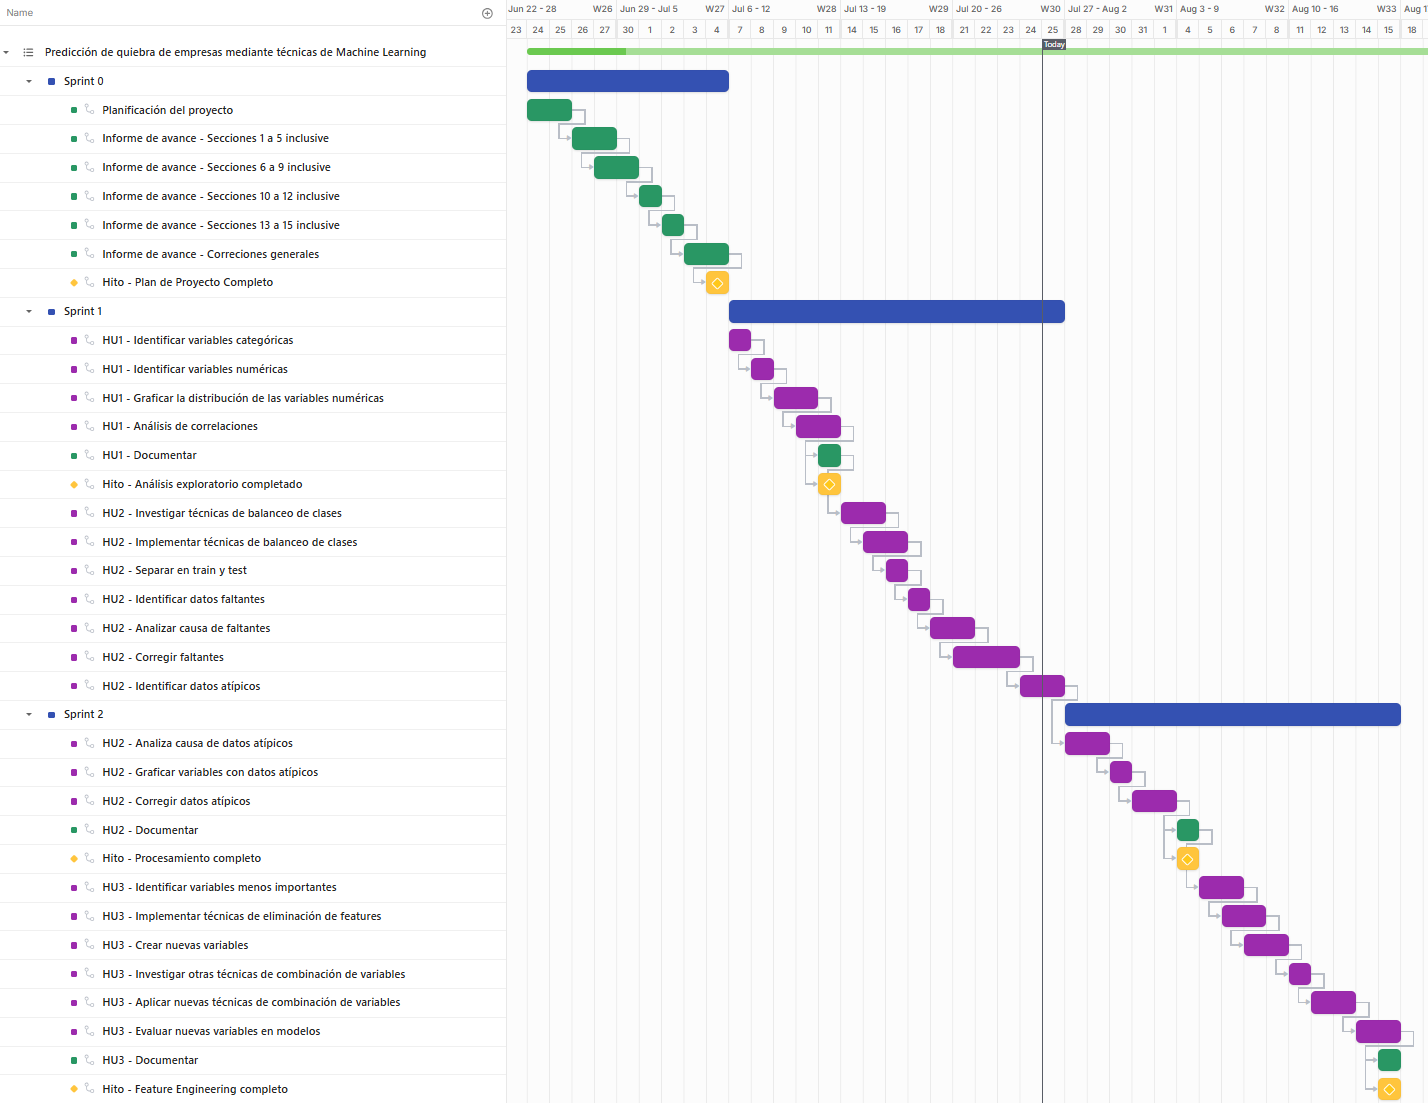
\includegraphics[width=1.2\textwidth]{./Figuras/Gantt-1.png}
\caption{Diagrama de Gantt - Sprints 0, 1 y 2}
\label{fig:gantt1}
\end{figure}
\end{landscape}

\begin{landscape}
\begin{figure}[htpb]
\centering 
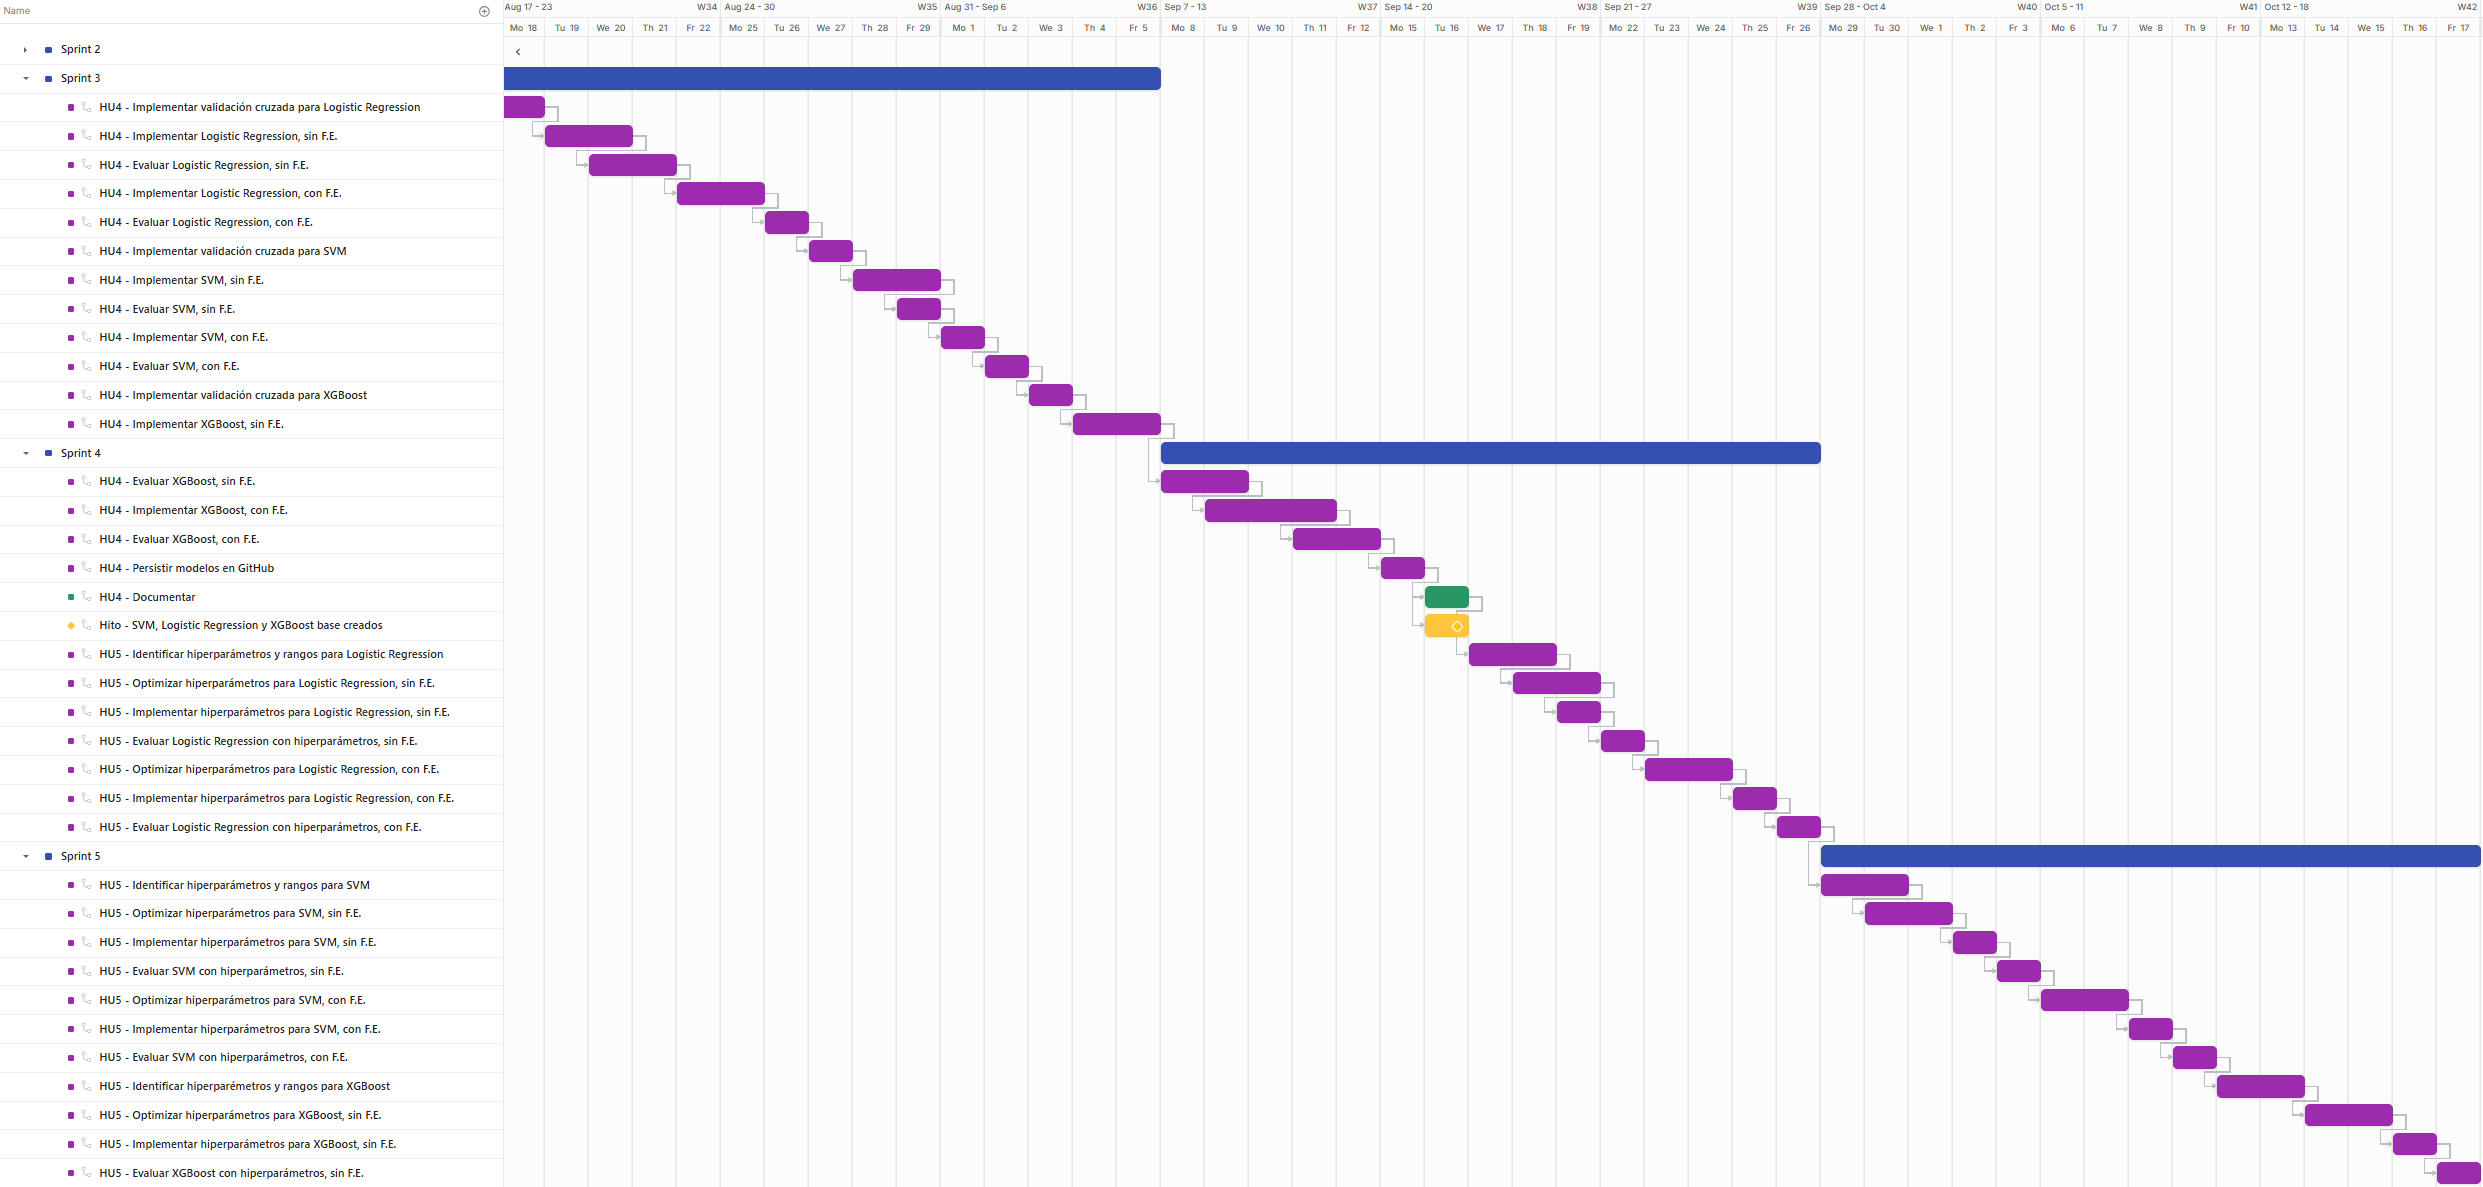
\includegraphics[width=1.5\textwidth]{./Figuras/Gantt-2.png}
\caption{Diagrama de Gantt - Sprints 3, 4 y 5}
\label{fig:gantt2}
\end{figure}
\end{landscape}

\begin{landscape}
\begin{figure}[htpb]
\centering 
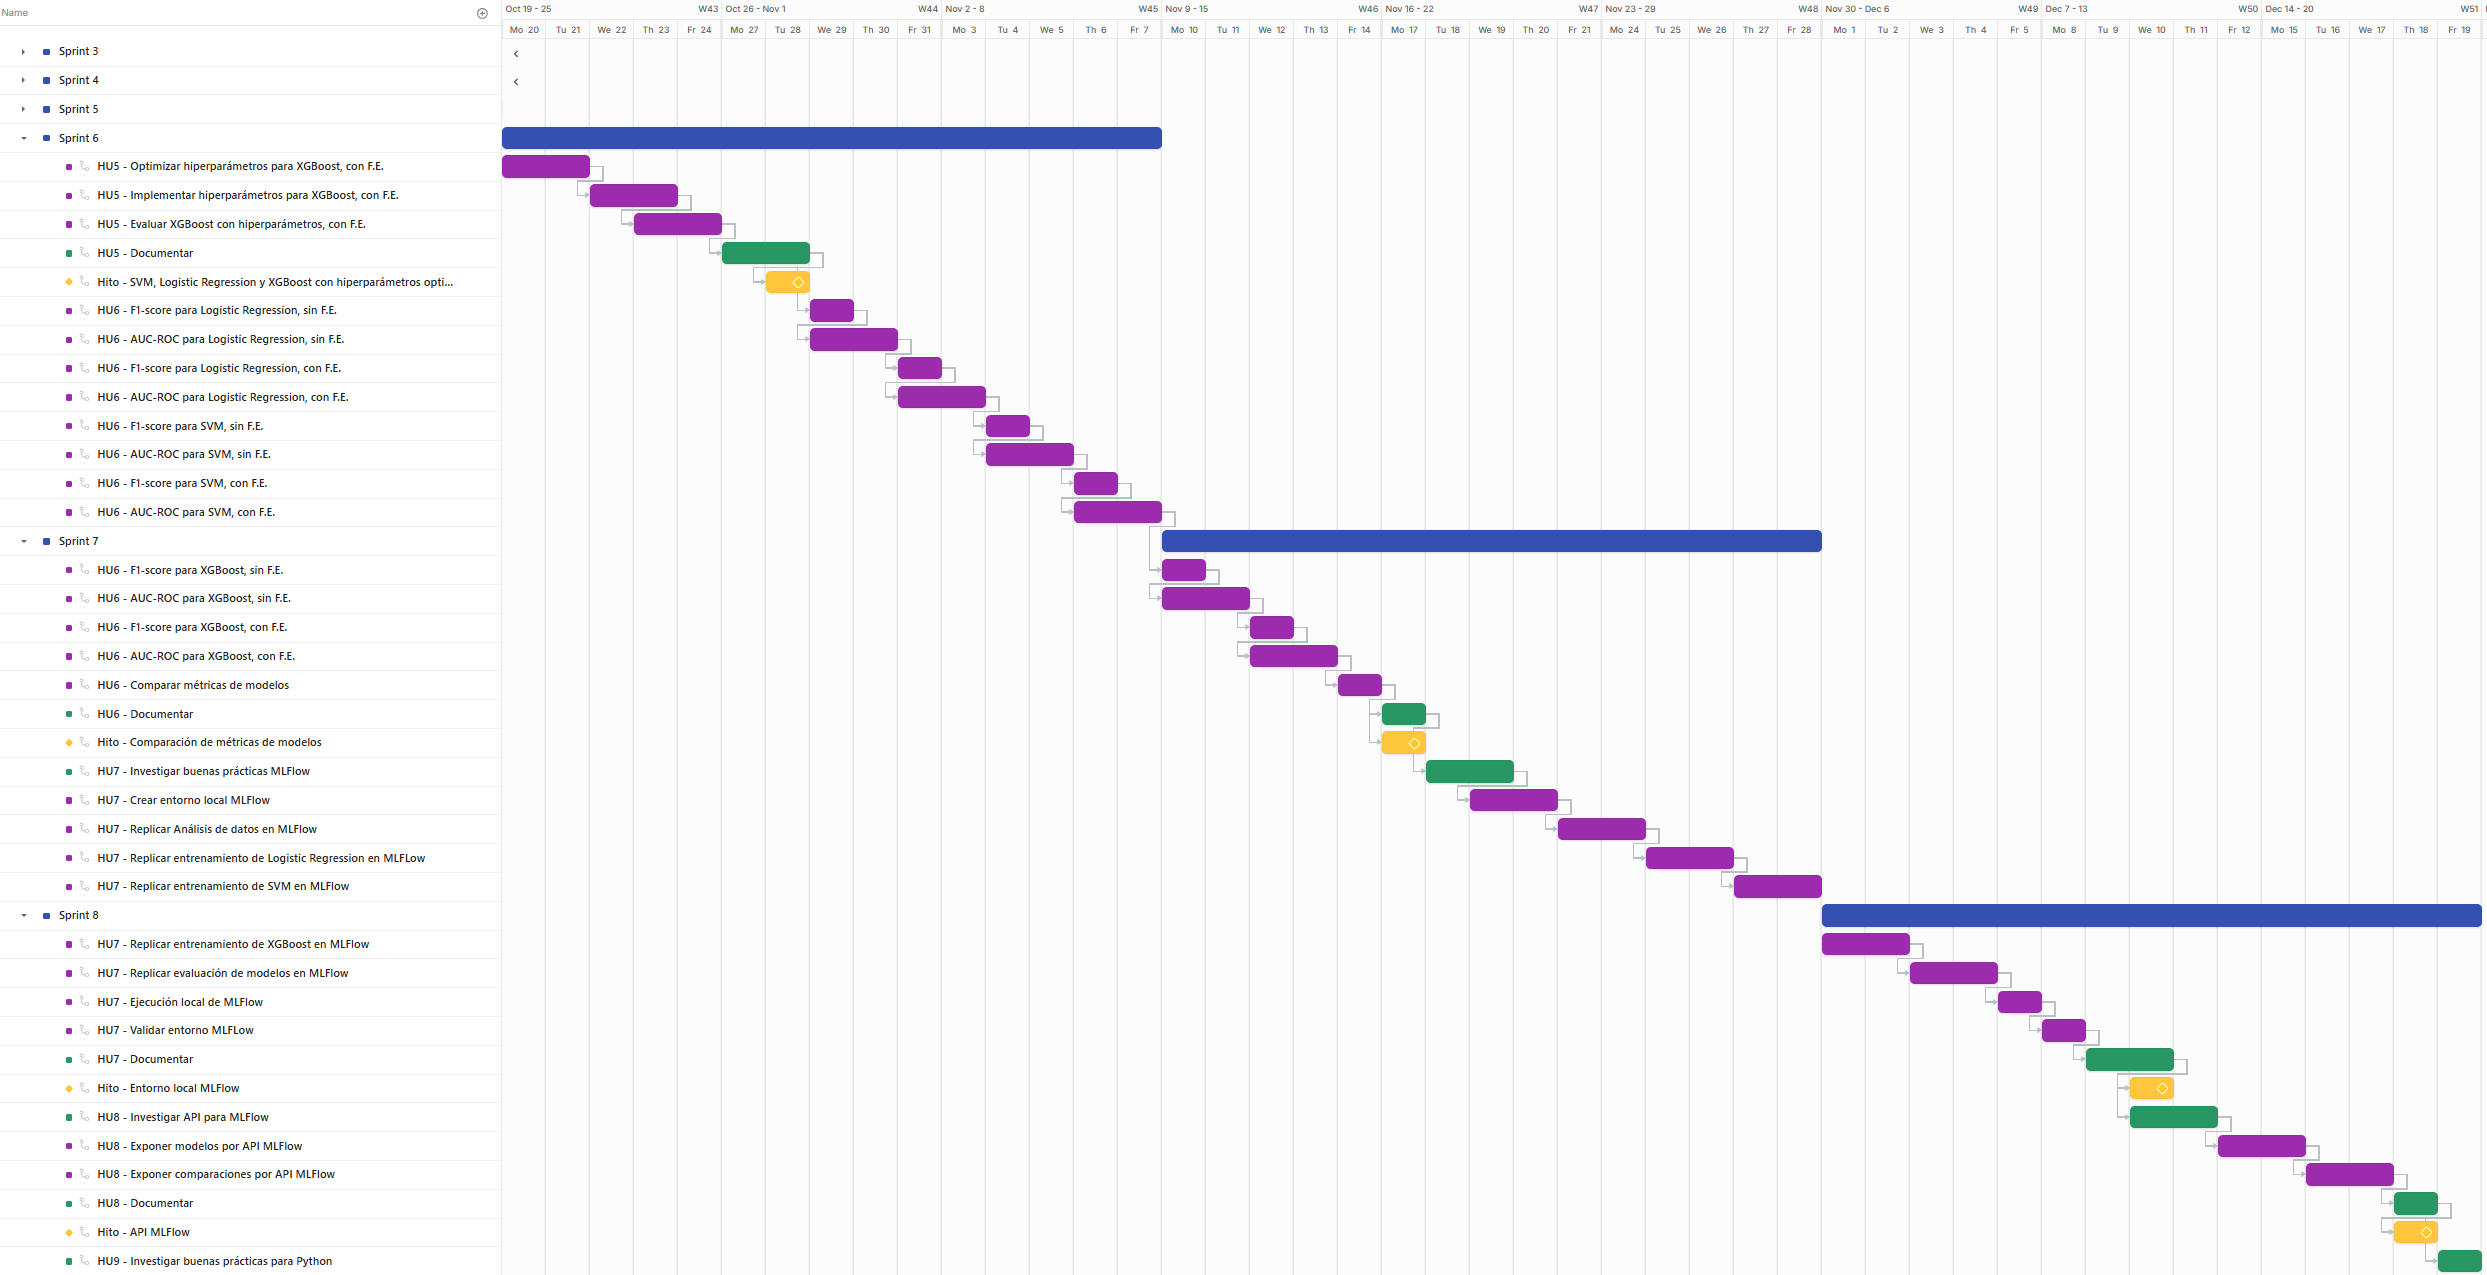
\includegraphics[width=1.5\textwidth]{./Figuras/Gantt-3.png}
\caption{Diagrama de Gantt - Sprints 6, 7 y 8}
\label{fig:gantt3}
\end{figure}
\end{landscape}

\begin{landscape}
\begin{figure}[htpb]
\centering 
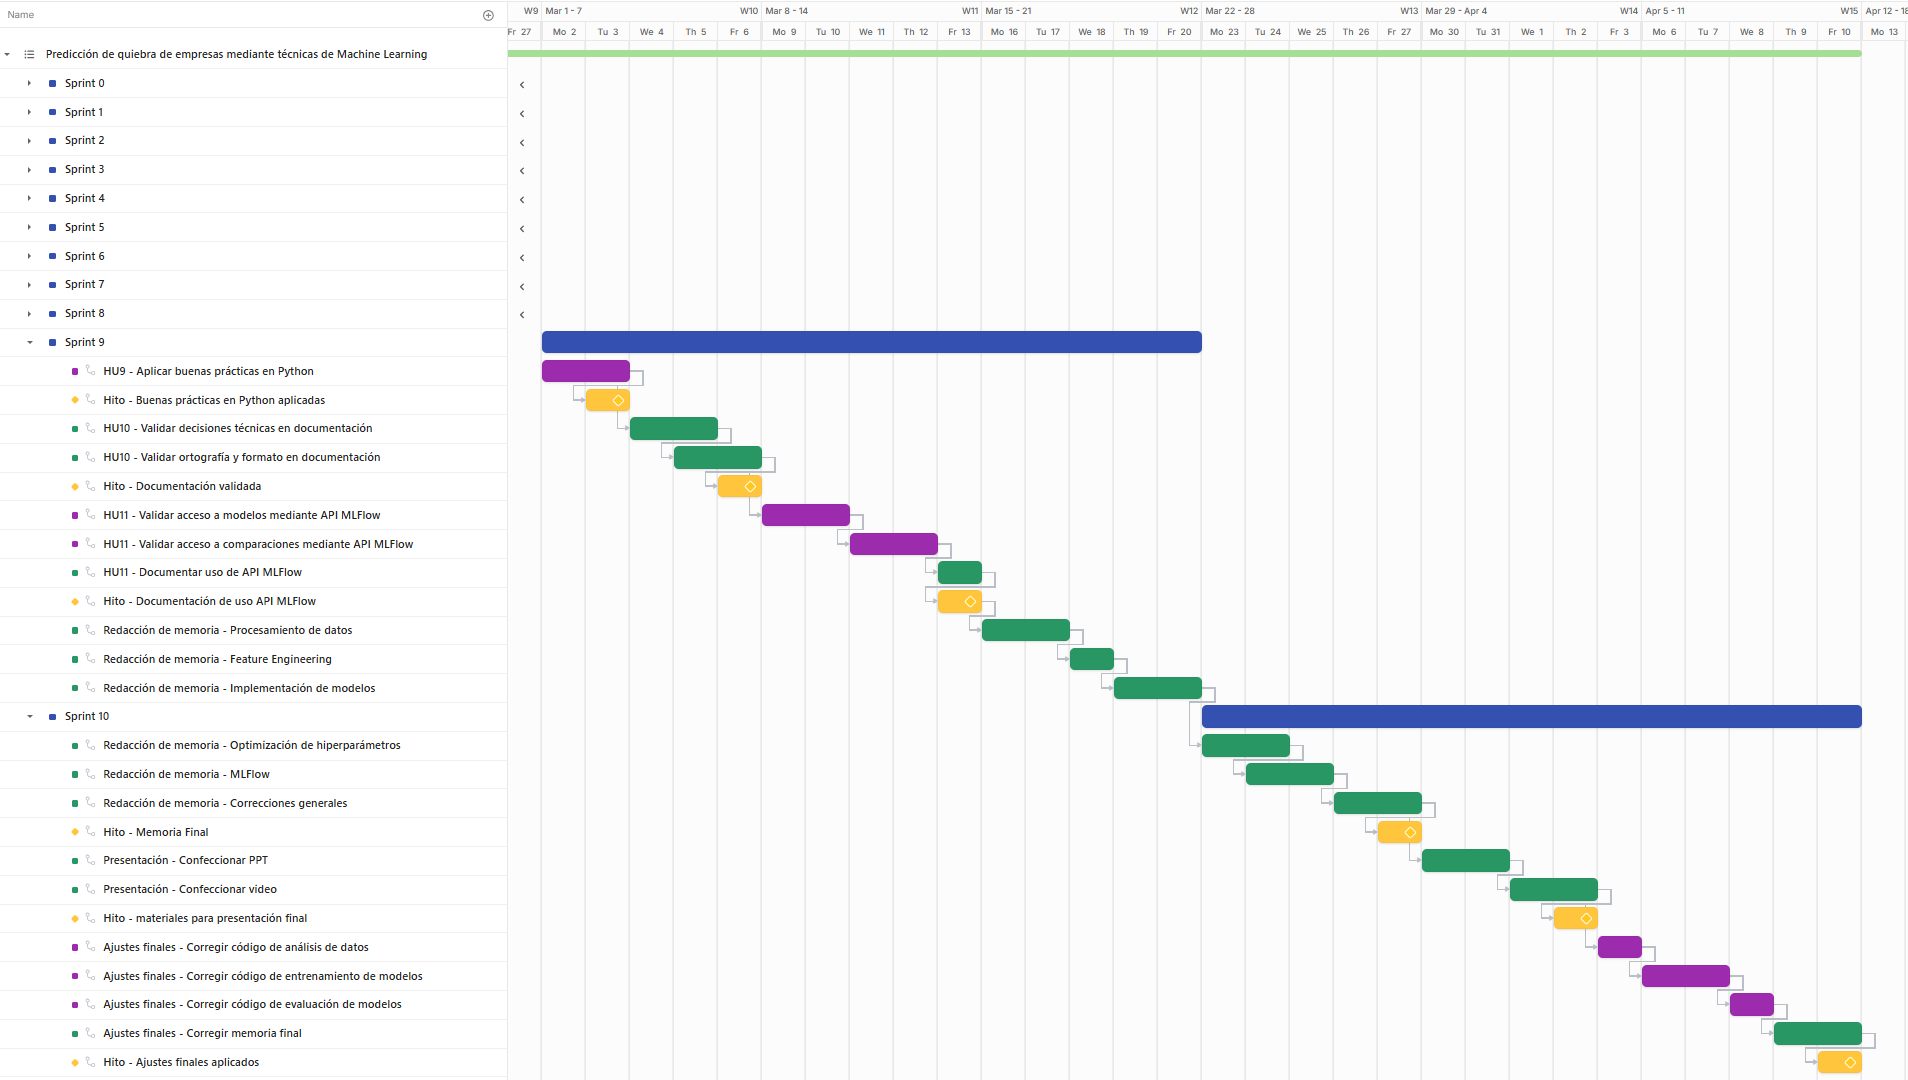
\includegraphics[width=1.5\textwidth]{./Figuras/Gantt-4.png}
\caption{Diagrama de Gantt - Sprints 9 y 10}
\label{fig:gantt4}
\end{figure}
\end{landscape}

\section{12. Normativa y cumplimiento de datos (gobernanza)}

%En esta sección se debe analizar si los datos utilizados en el proyecto están sujetos a normativas de protección de datos y privacidad, y en qué condiciones se pueden emplear.

%\textbf{Aspectos a considerar:}
%\begin{itemize}
%  \item Evaluar si los datos están regulados por normativas como GDPR, Ley 25.326 de Protección de Datos Personales en Argentina, HIPAA u otras según jurisdicción y temática.
%  \item Determinar si el uso de los datos requiere consentimiento explícito de los usuarios involucrados.
%  \item Indicar si existen restricciones legales, técnicas o contractuales sobre el uso, compartición o publicación de los datos.
%  \item Aclarar si los datos provienen de fuentes licenciadas, de acceso público o bajo algún tipo de autorización especial.
%  \item Analizar la viabilidad del proyecto desde el punto de vista legal y ético, considerando la gobernanza de los datos.
%\end{itemize}

%Este análisis es clave para garantizar el cumplimiento normativo y evitar conflictos legales durante el desarrollo y publicación del proyecto.

El proyecto utilizará el \textit{dataset} de \href{https://archive.ics.uci.edu/dataset/572/taiwanese+bankruptcy+prediction}{\textit{Taiwanese Bankruptcy Prediction}}.

El \textit{dataset} está publicado bajo la licencia \href{https://creativecommons.org/licenses/by/4.0/legalcode}{\textit{Creative Commons Attribution 4.0 International}}, la cual permite la copia, distribución, exhibición y ejecución de los datos siempre y cuando se dé crédito al autor y/o publicador, siendo en este caso el \href{https://archive.ics.uci.edu/}{repositorio de \textit{Machine Learning} de \textit{UC Irvine}}.

La información que presenta el \textit{dataset} fue recolectada y publicada por el \href{https://www.tejwin.com/en/}{Taiwan Economic Journal}. Tal como se menciona en la sección de \href{https://www.tejwin.com/en/solution/financial-data/}{\textit{financial data}} de su sitio web, todos los datos financieros que ellos presentan se obtienen de:
\begin{itemize}
    \item Informes auditados por contadores públicos certificados.
    \item Datos mensuales sobre ingresos proporcionados por empresas que cotizan en la bolsa de Taiwán
\end{itemize}

Como dato adicional, en el \textit{dataset} no se mencionan los nombres de las empresas ni datos similares, solo presenta información financiera.

Por todo lo mencionado anteriormente podemos garantizar que no hay inconvenientes al utilizar el \textit{dataset} de \href{https://archive.ics.uci.edu/dataset/572/taiwanese+bankruptcy+prediction}{\textit{Taiwanese Bankruptcy Prediction}} durante el desarrollo y publicación del proyecto. Solamente hay que dar crédito a su publicador (\href{https://archive.ics.uci.edu/}{repositorio de \textit{Machine Learning} de \textit{UC Irvine}}).

\section{13. Gestión de riesgos}
\label{sec:riesgos}

\begin{consigna}{red}
a) Identificación de los riesgos (al menos cinco) y estimación de sus consecuencias:
 
Riesgo 1: detallar el riesgo (riesgo es algo que si ocurre altera los planes previstos de forma negativa)
\begin{itemize}
	\item Severidad (S): mientras más severo, más alto es el número (usar números del 1 al 10).\\
	Justificar el motivo por el cual se asigna determinado número de severidad (S).
	\item Probabilidad de ocurrencia (O): mientras más probable, más alto es el número (usar del 1 al 10).\\
	Justificar el motivo por el cual se asigna determinado número de (O). 
\end{itemize}   

Riesgo 2:
\begin{itemize}
	\item Severidad (S): X.\\
	Justificación...
	\item Ocurrencia (O): Y.\\
	Justificación...
\end{itemize}

Riesgo 3:
\begin{itemize}
	\item Severidad (S):  X.\\
	Justificación...
	\item Ocurrencia (O): Y.\\
	Justificación...
\end{itemize}


b) Tabla de gestión de riesgos:      (El RPN se calcula como RPN=SxO)

\begin{table}[htpb]
\centering
\begin{tabularx}{\linewidth}{@{}|X|c|c|c|c|c|c|@{}}
\hline
\rowcolor[HTML]{C0C0C0} 
Riesgo & S & O & RPN & S* & O* & RPN* \\ \hline
       &   &   &     &    &    &      \\ \hline
       &   &   &     &    &    &      \\ \hline
       &   &   &     &    &    &      \\ \hline
       &   &   &     &    &    &      \\ \hline
       &   &   &     &    &    &      \\ \hline
\end{tabularx}%
\end{table}

Criterio adoptado: 

Se tomarán medidas de mitigación en los riesgos cuyos números de RPN sean mayores a...

Nota: los valores marcados con (*) en la tabla corresponden luego de haber aplicado la mitigación.

c) Plan de mitigación de los riesgos que originalmente excedían el RPN máximo establecido:
 
Riesgo 1: plan de mitigación (si por el RPN fuera necesario elaborar un plan de mitigación).
  Nueva asignación de S y O, con su respectiva justificación:
  \begin{itemize}
	\item Severidad (S*): mientras más severo, más alto es el número (usar números del 1 al 10).
          Justificar el motivo por el cual se asigna determinado número de severidad (S).
	\item Probabilidad de ocurrencia (O*): mientras más probable, más alto es el número (usar del 1 al 10).
          Justificar el motivo por el cual se asigna determinado número de (O).
	\end{itemize}

Riesgo 2: plan de mitigación (si por el RPN fuera necesario elaborar un plan de mitigación).
 
Riesgo 3: plan de mitigación (si por el RPN fuera necesario elaborar un plan de mitigación).

\end{consigna}

\section{14. Sprint Review}
\label{sec:sprint_review}

La revisión de sprint (\emph{Sprint Review}) es una práctica fundamental en metodologías ágiles. Consiste en revisar y evaluar lo que se ha completado al finalizar un sprint. En esta instancia, se presentan los avances y se verifica si las funcionalidades cumplen con los criterios de aceptación establecidos. También se identifican entregables parciales y se consideran ajustes si es necesario.

Aunque el proyecto aún se encuentre en etapa de planificación, esta sección permite proyectar cómo se evaluarán las funcionalidades más importantes del backlog. Esta mirada anticipada favorece la planificación enfocada en valor y permite reflexionar sobre posibles obstáculos.

\textbf{Objetivo:} anticipar cómo se evaluará el avance del proyecto a medida que se desarrollen las funcionalidades, utilizando como base al menos cuatro historias de usuario del \emph{Product Backlog}.


Seleccionar al menos 4 HU del Product Backlog. Para cada una, completar la siguiente tabla de revisión proyectada:

\textbf{Formato sugerido:}
\begin{table}[htpb]
\renewcommand{\arraystretch}{1.5}
\begin{tabular}{|>{\raggedright\arraybackslash}m{2.5cm}|
                >{\raggedright\arraybackslash}m{2.3cm}|
                >{\raggedright\arraybackslash}m{3cm}|
                >{\raggedright\arraybackslash}m{3cm}|
                >{\raggedright\arraybackslash}m{3cm}|}
\hline
\rowcolor[HTML]{CCCCCC}
\textbf{HU seleccionada} & \textbf{Tareas asociadas} & \textbf{Entregable esperado} & \textbf{¿Cómo sabrás que está cumplida?} & \textbf{Observaciones o riesgos} \\
\hline
                         & Tarea 1 &                             &                                           &                                     \\ \cline{2-2}
\multirow{-2}{=}{HU1}    & Tarea 2 & \multirow{-2}{=}{Módulo funcional} & \multirow{-2}{=}{Cumple criterios de aceptación definidos} & \multirow{-2}{=}{Falta validar con el tutor} \\
\hline
                         & Tarea 1 &                             &                                           &                                     \\ \cline{2-2}
\multirow{-2}{=}{HU3}    & Tarea 2 & \multirow{-2}{=}{Reporte generado} & \multirow{-2}{=}{Exportación disponible y clara} & \multirow{-2}{=}{Requiere datos reales} \\
\hline
                         & Tarea 1 &                             &                                           &                                     \\ \cline{2-2}
\multirow{-2}{=}{HU5}    & Tarea 2 & \multirow{-2}{=}{Panel de gestión} & \multirow{-2}{=}{Roles diferenciados operativos} & \multirow{-2}{=}{Riesgo en integración} \\
\hline
                         & Tarea 1 &                             &                                           &                                     \\ \cline{2-2}
\multirow{-2}{=}{HU7}    & Tarea 2 & \multirow{-2}{=}{Informe trimestral} & \multirow{-2}{=}{PDF con gráficos y evolución} & \multirow{-2}{=}{Puede faltar tiempo para ajustes} \\
\hline
\end{tabular}
\end{table}

\section{15. Sprint Retrospective}    
\label{sec:sprint_retro}

La retrospectiva de sprint es una práctica orientada a la mejora continua. Al finalizar un sprint, el equipo (o el alumno, si trabaja de forma individual) reflexiona sobre lo que funcionó bien, lo que puede mejorarse y qué acciones concretas pueden implementarse para trabajar mejor en el futuro.

Durante la cursada se propuso el uso de la \textbf{Estrella de la Retrospectiva}, que organiza la reflexión en torno a cinco ejes:

\begin{itemize}
\item  ¿Qué hacer más?
\item  ¿Qué hacer menos?
\item  ¿Qué mantener?
\item  ¿Qué empezar a hacer?
\item  ¿Qué dejar de hacer?
\end{itemize}

Aun en una etapa temprana, esta herramienta permite que el alumno planifique su forma de trabajar, identifique anticipadamente posibles dificultades y diseñe estrategias de organización personal.

\textbf{Objetivo:} reflexionar sobre las condiciones iniciales del proyecto, identificando fortalezas, posibles dificultades y estrategias de mejora, incluso antes del inicio del desarrollo.


Completar la siguiente tabla tomando como referencia los cinco ejes de la Estrella de la Retrospectiva (\emph{Starfish} o estrella de mar). Esta instancia te ayudará a definir buenas prácticas desde el inicio y prepararte para enfrentar el trabajo de forma organizada y flexible. Se deberá completar la tabla al menos para 3 sprints técnicos y 1 no técnico.

\textbf{Formato sugerido:}

\begin{table}[htpb]
\renewcommand{\arraystretch}{1.4}
\begin{tabular}{|>{\raggedright\arraybackslash}p{1.8cm}|
                >{\raggedright\arraybackslash}p{2.3cm}|
                >{\raggedright\arraybackslash}p{2.3cm}|
                >{\raggedright\arraybackslash}p{2.3cm}|
                >{\raggedright\arraybackslash}p{2.3cm}|
                >{\raggedright\arraybackslash}p{2.3cm}|}
\hline
\rowcolor[HTML]{CCCCCC} 
\textbf{Sprint tipo y N°} & \textbf{¿Qué hacer más?} & \textbf{¿Qué hacer menos?} & \textbf{¿Qué mantener?} & \textbf{¿Qué empezar a hacer?} & \textbf{¿Qué dejar de hacer?} \\
\hline
Sprint técnico - 1 & Validaciones continuas con el alumno & Cambios sin versión registrada & Pruebas con datos simulados & Documentar cambios propuestos & Ajustes sin análisis de impacto \\
\hline
Sprint técnico - 2 & Verificar configuraciones en múltiples escenarios & Modificar parámetros sin guardar historial & Perfiles reutilizables & Usar logs para configuración & Repetir pruebas manuales innecesarias \\
\hline
Sprint técnico - 8 & Comparar correlaciones con casos previos & Cambiar parámetros sin justificar & Revisión cruzada de métricas & Anotar configuraciones usadas & Trabajar sin respaldo de datos \\
\hline
Sprint no técnico - 12 (por ej.: ``Defensa'') & Ensayos orales con feedback & Cambiar contenidos en la memoria & Material visual claro & Dividir la presentación por bloques & Agregar gráficos difíciles de explicar \\
\hline
\end{tabular}
\end{table}




\end{document}